%----------------------------------------------------------------------------------------
%	PACKAGES AND OTHER DOCUMENT CONFIGURATIONS
%----------------------------------------------------------------------------------------

\documentclass[12pt]{article}
\renewcommand{\contentsname}{whatever}
\renewcommand{\refname}{whatever}
\usepackage[danish]{babel}
\usepackage{mathtools}
\usepackage[euler]{textgreek}
\usepackage[numbered,final]{mcode}
\usepackage[utf8x]{inputenc}
\usepackage{amsmath}
\usepackage{graphicx}
\usepackage[colorinlistoftodos]{todonotes}
\usepackage[toc,page]{appendix}
%\usepackage{float}
\usepackage{floatrow} % used for adding "Source" to pictures
\usepackage{hyperref} % used for hyperlinks
\usepackage[all]{hypcap}
 \usepackage{bm} % used for bold inline matj
\usepackage{lipsum} % used for lorem lipsum
\usepackage[final]{pdfpages} % used for including PDF's
\usepackage{geometry}
\usepackage{listingsutf8}
\usepackage{listings}
\usepackage{helvet}					% Using Helvetica font
\usepackage[parfill]{parskip}		% Removes indention of first line in paragraph

\usepackage{color} %red, green, blue, yellow, cyan, magenta, black, white
% Define colors
\definecolor{Blue}{RGB}{56,85,96}			
\definecolor{Grey}{RGB}{145,145,145}
\usepackage{multirow}

\usepackage{colortbl}
\usepackage{multicol}
\hypersetup{colorlinks=true, linkcolor=black}

% Page margins
\geometry{verbose,tmargin=1in,bmargin=1in,lmargin=1in,rmargin=1in,headsep=0.35in}


\begin{document}
	
	\begin{titlepage}
		
		
		
		\newcommand{\HRule}{\rule{\linewidth}{0.5mm}} % Defines a new command for the horizontal lines, change thickness here
		\setlength{\topmargin}{0in}
		\centering % Center everything on the page
		
		%----------------------------------------------------------------------------------------
		%	HEADING SECTIONS
		%----------------------------------------------------------------------------------------
		\textsc{\LARGE Aarhus School of Engineering}\\[1.5cm] % Name of your university/college
		\textsc{\Large Anvendte Microcontroller Systemer}\\[0.5cm] % Major heading such as course name
		\textsc{\large 6. Semester}\\[0.5cm] % Minor heading such as course title
		
		%----------------------------------------------------------------------------------------
		%	TITLE SECTION
		%----------------------------------------------------------------------------------------
		
		\HRule \\[0.4cm]
		{ \huge \bfseries AMS projekt}\\ % Title of your document
		\HRule \\[1cm]
		
		%----------------------------------------------------------------------------------------
		%	AUTHOR SECTION
		%----------------------------------------------------------------------------------------
		
		\begin{minipage}{0.4\textwidth}
			\begin{flushleft} \large
				\emph{Gruppemedlemmer:}\\
				Søren Landgrebe \\
				Philip Nygaard Scmhidt \\
			\end{flushleft}
		\end{minipage}
		~
		\begin{minipage}{0.4\textwidth}
			\begin{flushright} \large
				\emph{Studienr:} \\
				201508295\\
				201506381\\
			\end{flushright}
		\end{minipage}\\[5cm]
		
		%----------------------------------------------------------------------------------------
		%	LOGO SECTION
		%----------------------------------------------------------------------------------------
		
		
\includegraphics[scale=0.5]{Img/logo.jpg}\\[1cm]
		
		%----------------------------------------------------------------------------------------
		%	DATE SECTION
		%----------------------------------------------------------------------------------------
		{\large \today}\\[0.5cm] % Date, change the \today to a set date if you want to be precise
		
		
		\vfill % Fill the rest of the page with whitespace
		
	\end{titlepage}
	
\newpage
\tableofcontents
\newpage
\listoffigures
\newpage

\hypersetup{linkcolor=blue}



%!TEX root = ../../Main.tex
\graphicspath{{Chapters/Indledning/}}
%-------------------------------------------------------------------------------

\section{Indledning}
Næsten alle danskere har nu til dags en smartphone med indbygget Bluetooth modul, som man altid har med på sig, når man forlader sit hjem. Dette vil gruppen gerne udnytte til at kunne gøre det nemmere for brugere, at kunne låse op og låse hoveddøren, som adskiller omverdenen fra ens dyrebare ejendele. Dette betyder at forbrugeren aldrig skal tænke mere på nøgler, da disse bliver overflødige. Hermed slipper brugeren for at skulle huske på dette, samt at skulle fumle med nøglerne når man kommer hjem med flere poser i hænderne fra dagens indkøbstur. 

\begin{figure}[H]
	\centering
	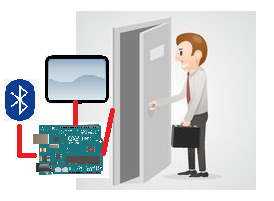
\includegraphics[width = 300 pt]{Img/Konceptbillede.png}
	\caption{Konceptbillede}
	\label{fig:Konceptbillede}
\end{figure}

	%!TEX root = ../../Main.tex
\graphicspath{{Chapters/Krav/}}
%-------------------------------------------------------------------------------


\section{Krav}
I dette afsnit beskrives kravene til hvilken funktionalitet systemet har. 


I samarbejde med vejleder er der opstillet en række krav.
\begin{itemize}
\item Systemet skal kunne finde de 4 stærkeste bluetooth signaler. 
\item Systemet skal kunne køre "hele tiden"
\item Systemet skal opdateres en gang i hvert sekund.  
\end{itemize}


%!TEX root = ../../Main.tex
\graphicspath{{Chapters/System/}}
%-------------------------------------------------------------------------------


\section{System beskrivelse}

BA-TA's (Bluetooth Anti-Theft Alarm) primære funktionalitet ligger i hhv. at kunne låse op og låse hoveddøren, så snart systemet registrerer at husets ejer (og dermed smartphone) eller en anden godkendt Bluetooth-enhed, er i nærheden eller ej.

Igennem brugergrænsefladen kan brugeren både tilføje og fjerne de godkendte Bluetooth-enheder (personer) som skal kunne låse og låse op for døren.

Når alle godkendte enheder er uden for rækkevidde af systemets Bluetooth-modul, låses døren, og så snart systemet ser en godkendt enhed indenfor rækkevidden bliver døren igen låst op. 

I under-afsnittende herunder bliver systemets blokke og de interne fobindelser præsenteret.
På figur \ref{fig:Bdd} ses et overordnet Bdd for projektet, hvor de interne forbindelser forklares på figur \ref{fig:Ibd}. 

\begin{figure}[H]
	\centering
	\includegraphics[width = 500 pt]{Img/Bdd.png}
	\caption{Bdd af BA-TA}
	\label{fig:Bdd}
\end{figure}

\subsection{Blokbeskrivelse BA-TA}
\textbf{Arduino} \\*
Arduino'en, mega2560, initialiserer og styrer alt funktionaliteten som indgår i systemet. Arduino blokken står for at initialisere  Touch Display, Touch Controller og Display Controller som bruges til at kunne modtage signaler fra Touch-delen, samt at sende signaler til Display'et og dermed få repræsenteret noget til brugeren. Yderligere bruges Arduinoen til at initialisere og kontrollere UART driveren og Bluetooth modulet.
\newline
\newline
\textbf{Touch Controller} \\*
Touch Controller står for at modtage værdier fra Touch Display, samt at sende den modtagede værdi videre til Arduino'en. 
\newline
\newline
\textbf{Display Controller} \\*
Display Controller modtager værdier fra Arduino'en og sende sende værdien videre til Touch Display. \newline
\newline
\textbf{Bluetooth} \\*
Bluetooth modul, HC-05, som kommunikkerer med Arduino'en vha. AT-kommandoer.
\newline
\newline
\textbf{Touch Display} \\*
Touch Display fungerer som brugergrænseflade og er dermed måden brugeren kan interagere med systemet. 
\newline
\newline
\textbf{Lock} \\*
Lock er den fysiske lås, denne er ikke implementeret i projektet, men simuleres med en visuel lås på skærmen. 
\subsection{Internal Block Diagram for BA-TA}
På figur \ref{fig:Ibd} ses et overordnet IBD over selve systemet, som er bygget på Bdd'et. 
\begin{figure}[H]
	\centering
	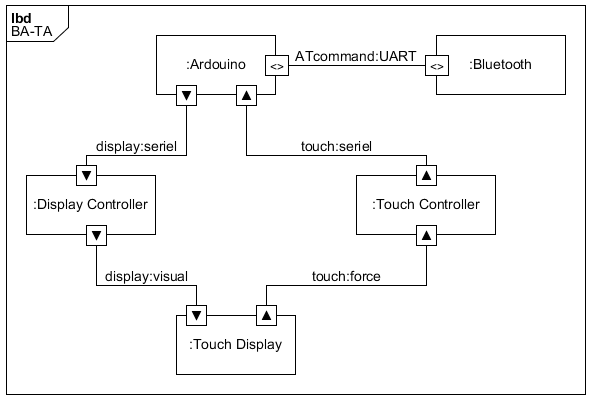
\includegraphics[width = 300 pt]{Img/Ibd.png}
	\caption{Ibd af BA-TA}
	\label{fig:Ibd}
\end{figure}




%!TEX root = ../../Main.tex
\graphicspath{{Chapters/SystemArkitektur/}}
%-------------------------------------------------------------------------------

\section{System Arkitektur}

Se under vores PRJ4 rapport.
Herunder plejer der at være følgende:


ENTITY diagram
Sekvens diagrammer
Andre relevante diagrammer

Opremsning af moduler, deres rolle, samt kommunikationsprotokoller


System arkitektur er jo en måde at forklare hvordan strukturenen i systemet og måden det opfører sig på.
	%!TEX root = ../../Main.tex
\graphicspath{{Chapters/Userinterface/}}
%-------------------------------------------------------------------------------


\section{Brugergrænseflade}
I dette afsnit gives der et overblik over brugergrænsefladen og brugerens mulighed for interaktion med denne. Afsnittet er bygget op af billeder, hvor hvert billede viser brugergrænsefladens visuelle struktur. \\

Første display man møder er "Welcome". Her går systemet igang med at initialisere de forskellige moduler og drivere, således de er klar til brug.
\begin{figure}[H]
	\centering
	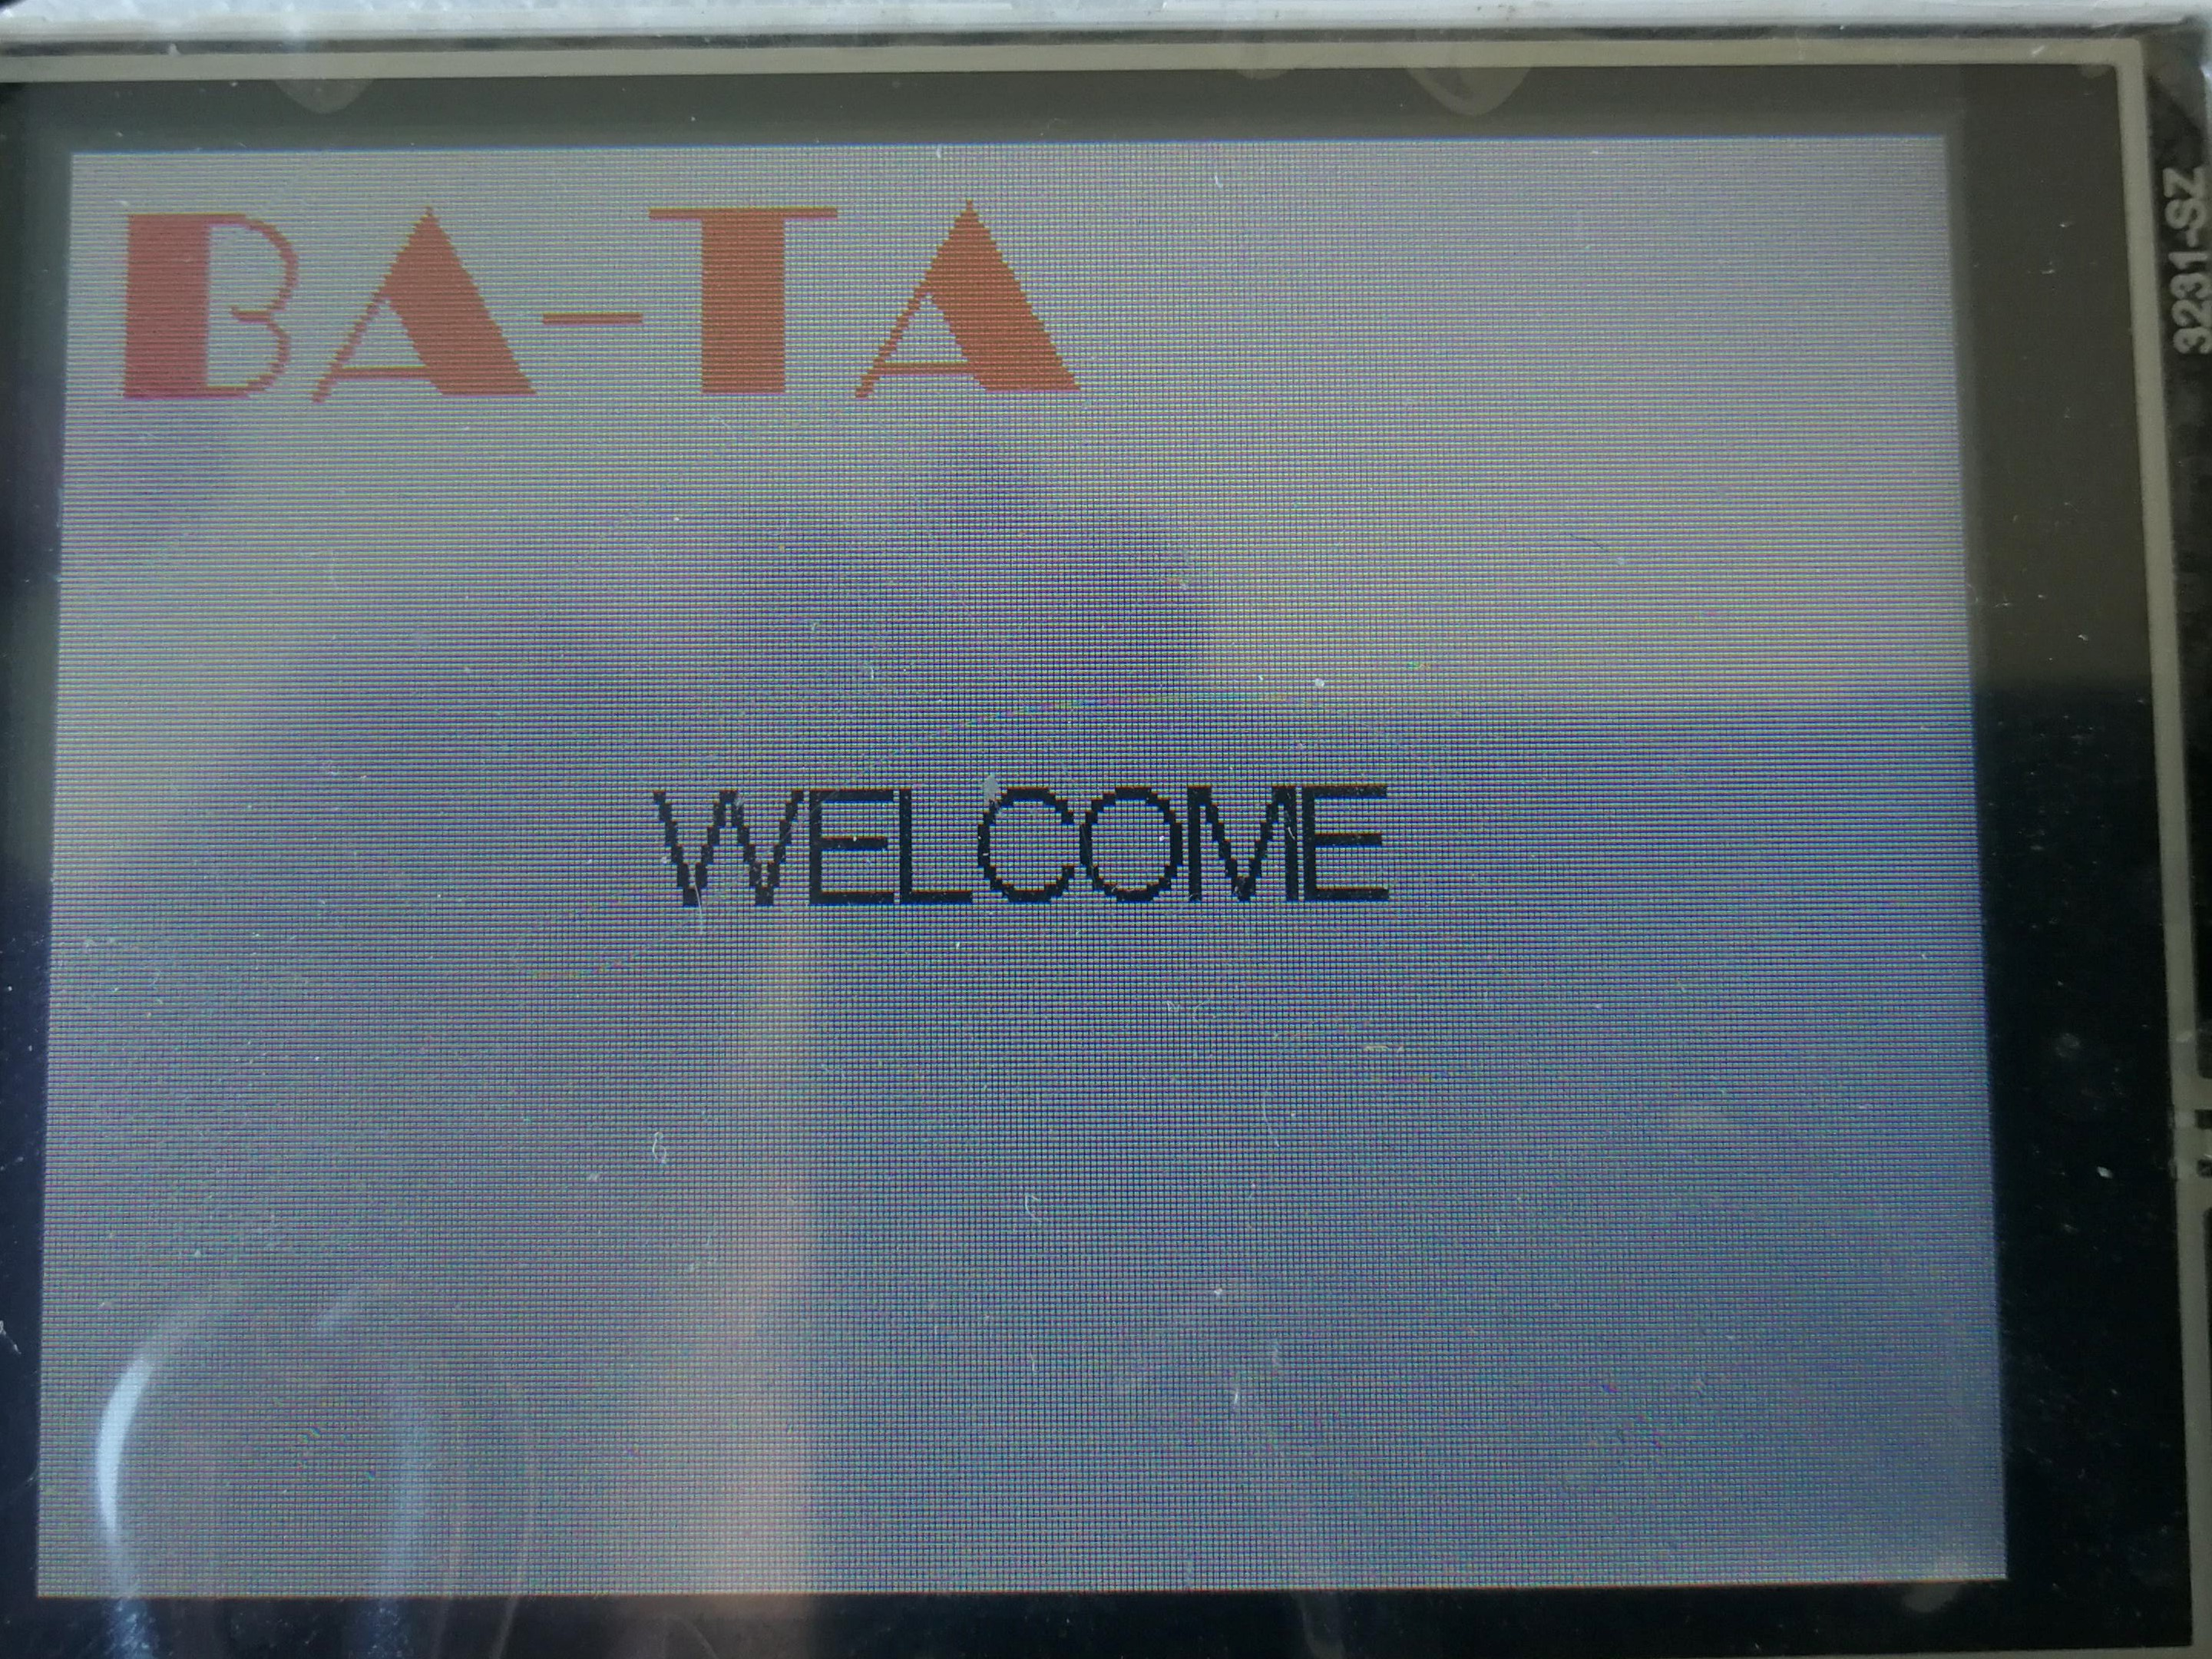
\includegraphics[width = 300 pt]{Img/welcome.jpg}
	\caption{Brugergrænseflade: Welcome}
	\label{fig:welcome}
\end{figure}

Næste display er hovedmenuen for systemet, hvor der er tre forskellige muligheder, som ses på figur     \ref{fig:start}. Yderligere ses der 4 trykknapper, hvor brugeren kan interagere med systemet.

\begin{itemize}  
	\item  Med "Enter" vælger brugeren en funktion
	\item "Back" gør brugeren i stand til at gå tilbage til hovedmenuen, hvis man forinden har trykket "ENTER" ved "ADD DEVICE" eller "REMOVE DEVICE".
	\item "Up" og "Down" flytter pilen, hhv. op og ned.
\end{itemize}

 Herudover ses der en farvet boks øverst i højre hjørne, som indikerer låsens tilstand. Denne lås viser grøn ved låst op og rød ved låst. Øverst til venstre på skærmen vises systemets logo.    
\begin{figure}[H]
	\centering
	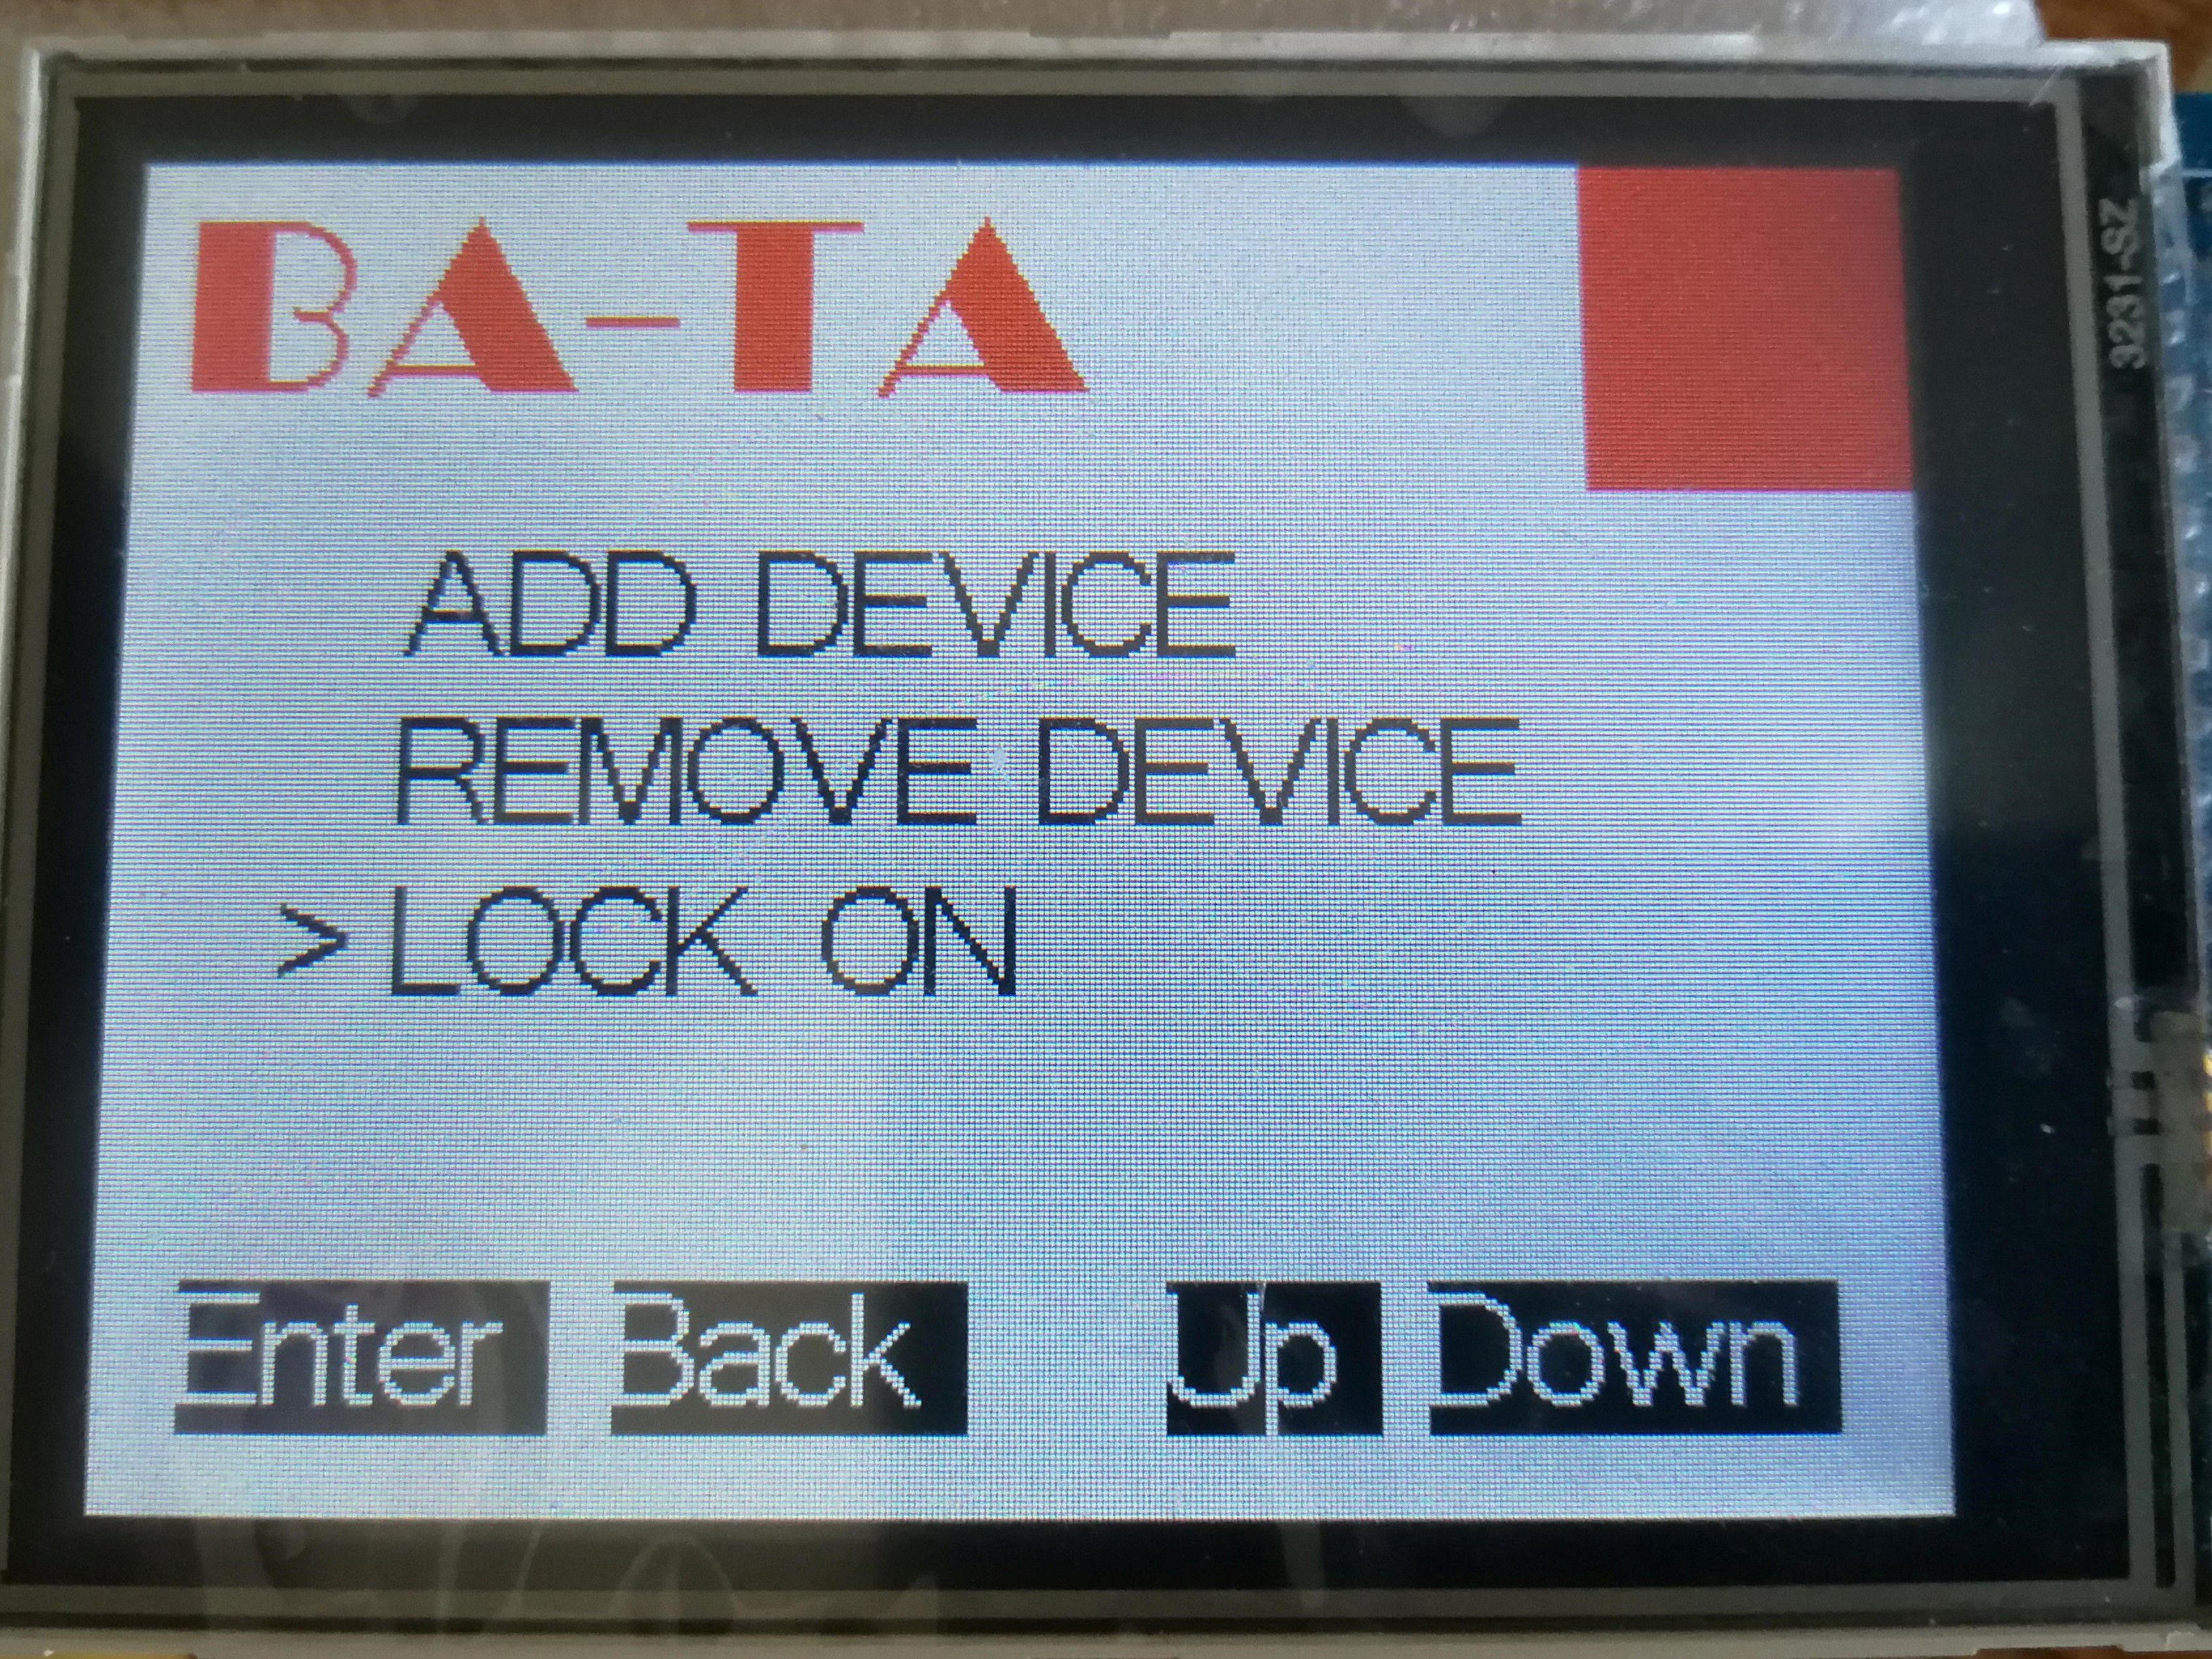
\includegraphics[width = 300 pt]{Img/start.jpg}
	\caption{Brugergrænseflade: Hovedmenu}
	\label{fig:start}
\end{figure}

Hvis brugeren trykker på "ADD DEVICE", søger BA-TA efter de 4 stærkeste Bluetooth signaler, som er indenfor rækkevidde. 
\begin{figure}[H]
	\centering
	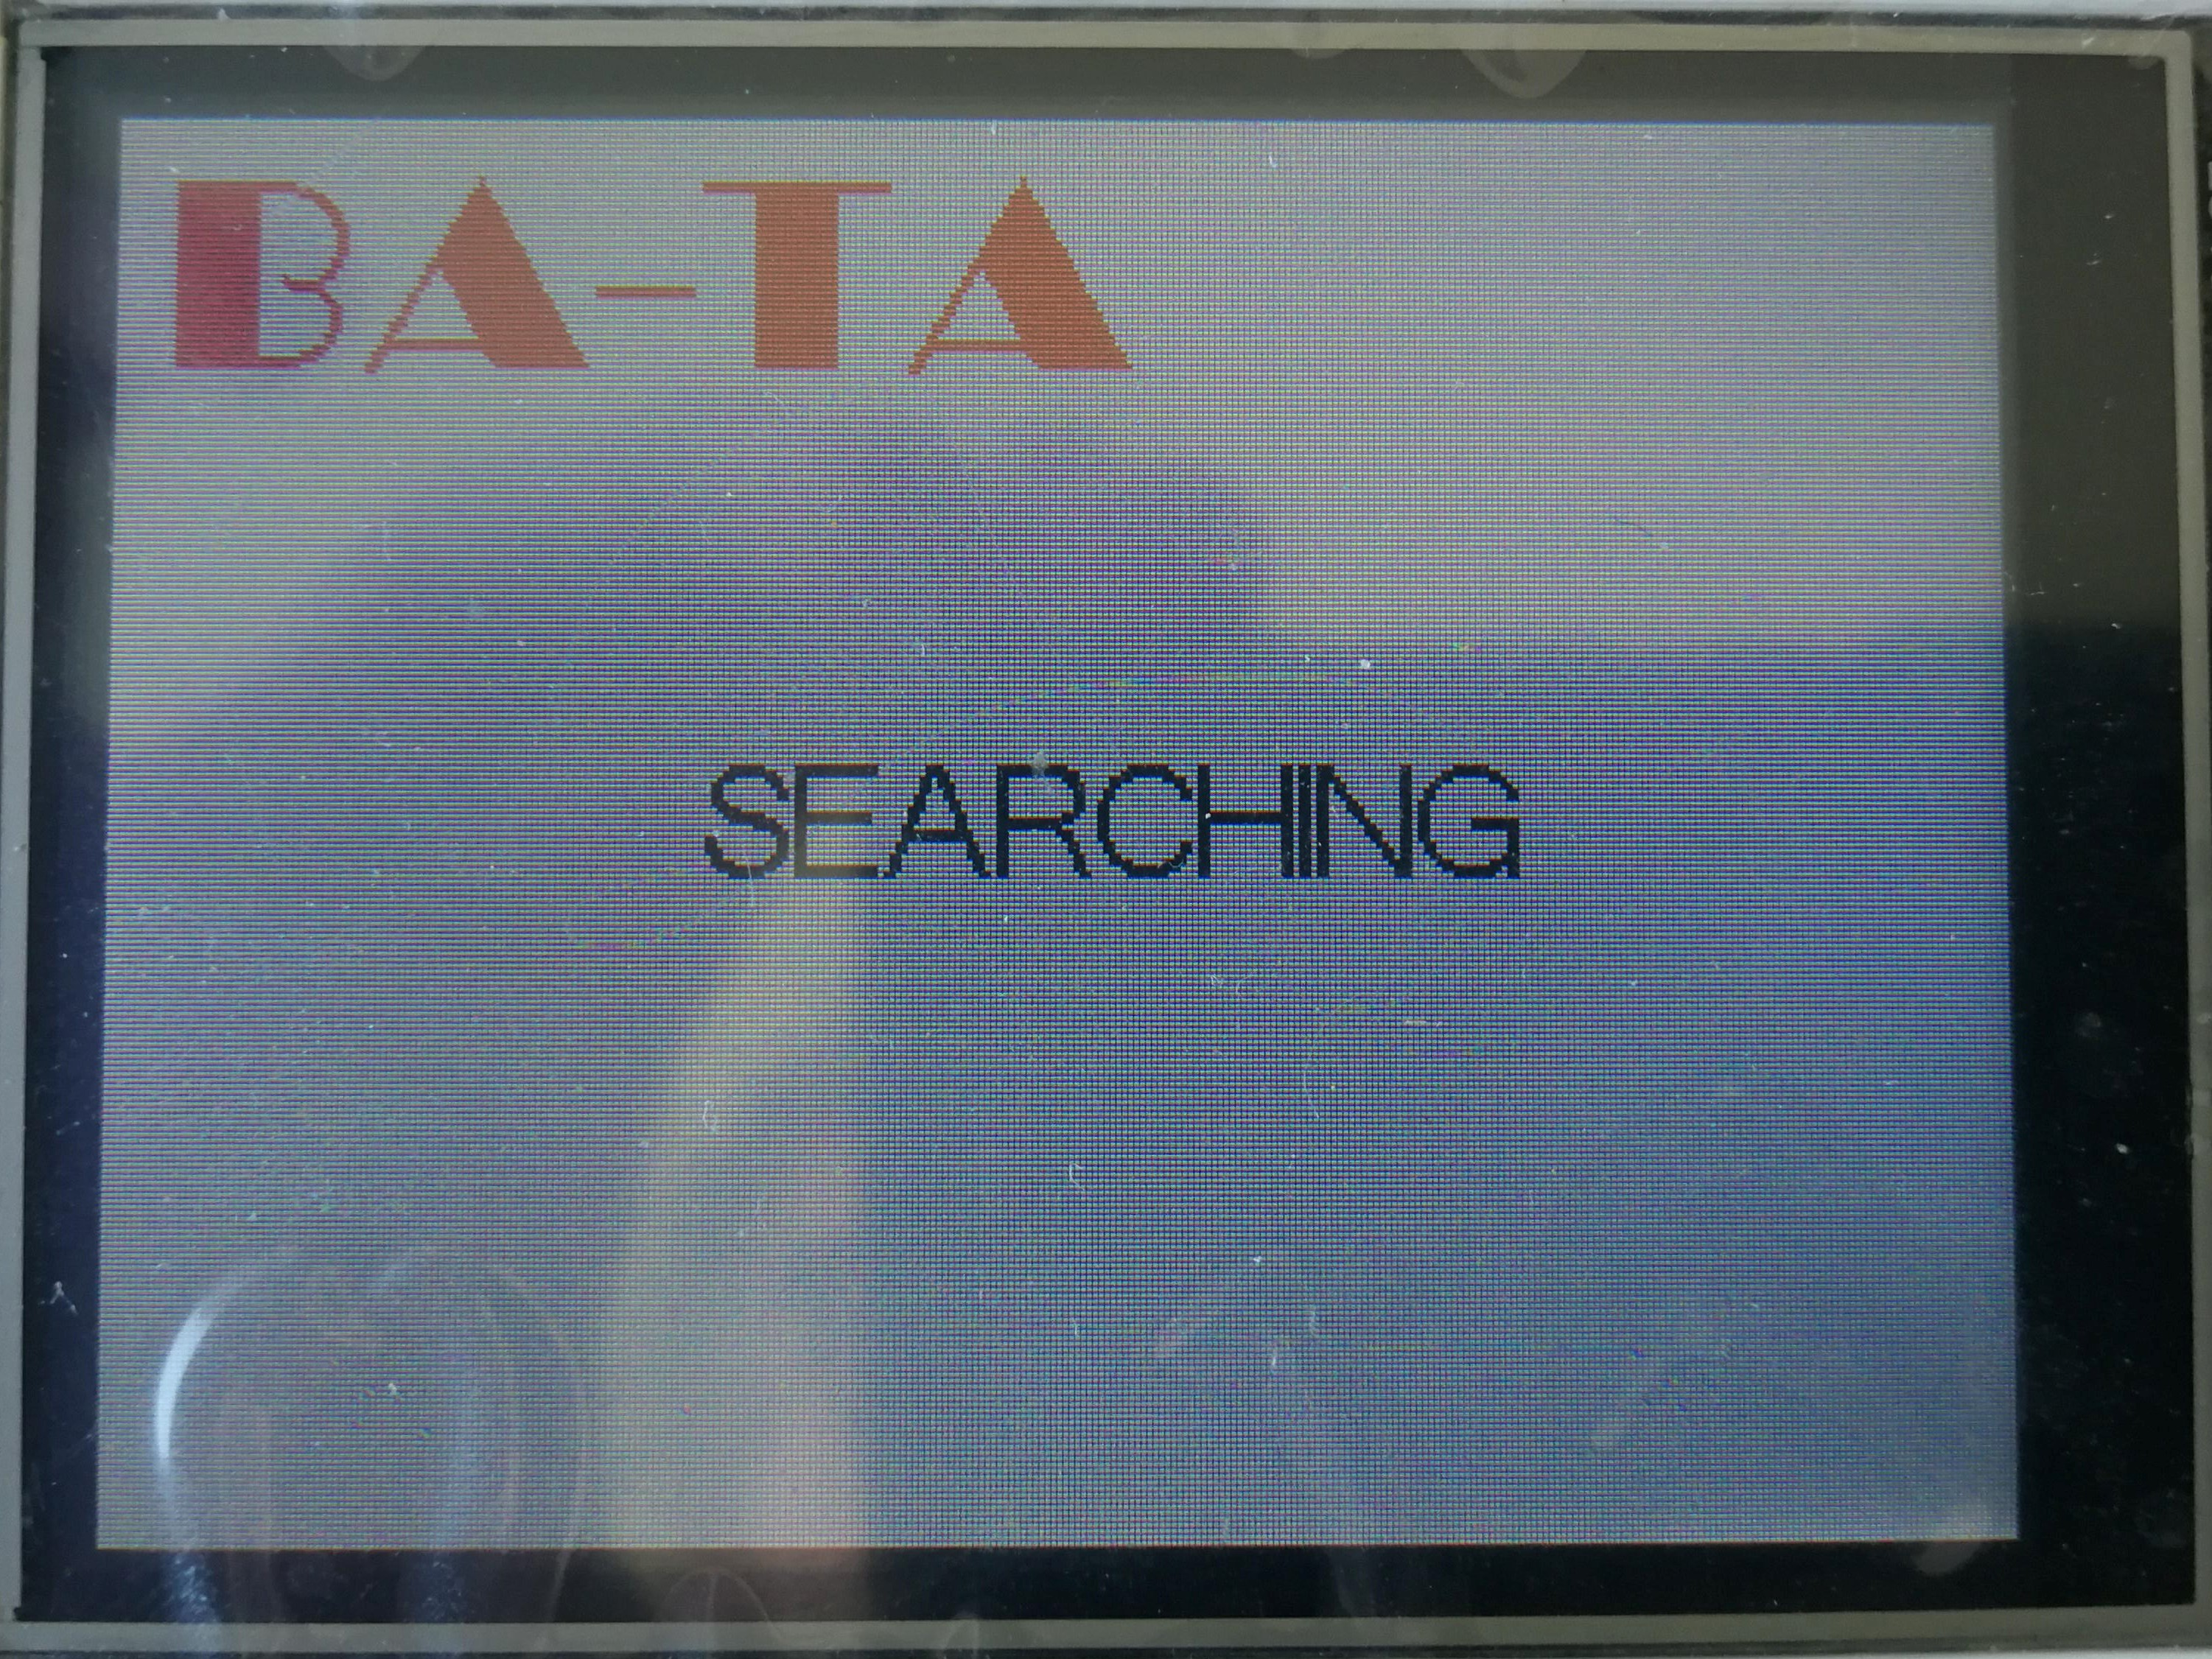
\includegraphics[width = 300 pt]{Img/Searching.jpg}
	\caption{Brugergrænseflade: Searching}
	\label{fig:Searching}
\end{figure}
Herefter vises de fundne Bluetooth-enheder, som systemets Bluetooth-modul har fundet. Dette ses på figur \ref{fig:devices}.
\begin{figure}[H]
	\centering
	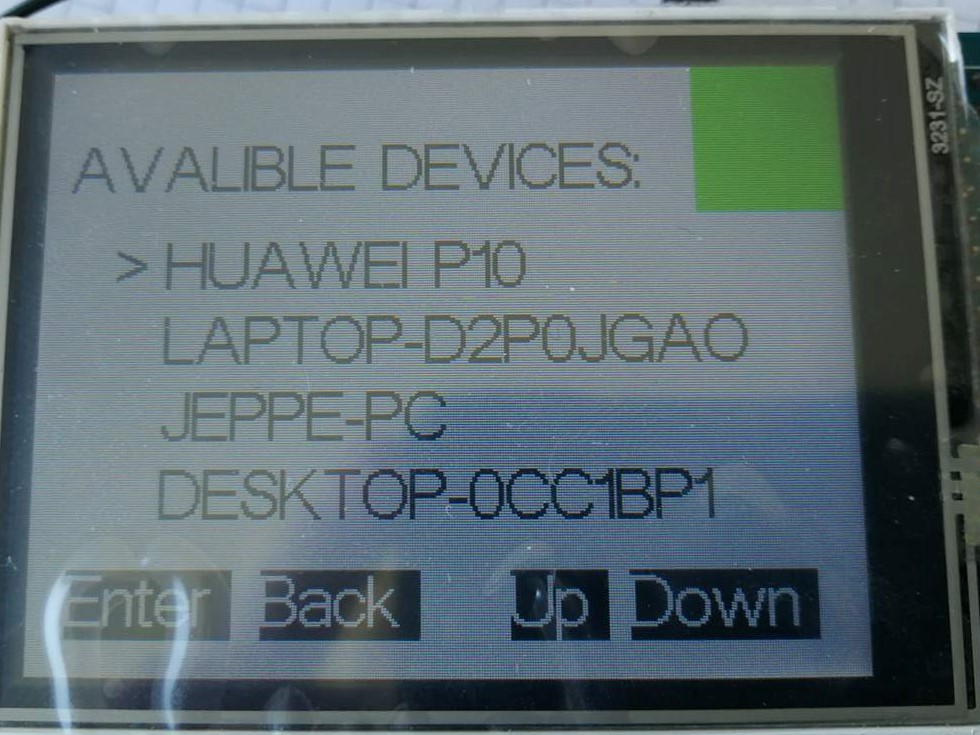
\includegraphics[width = 300 pt]{Img/devices.jpg}
	\caption{Brugergrænseflade: Tilgængelige enheder}
	\label{fig:devices}
\end{figure}
Hvis der vælges en enhed ved et tryk på "Enter", så vises navnet på den valgte enhed. Herefter går skærmens tilstand tilbage til hovedmenuen. 
\begin{figure}[H]
	\centering
	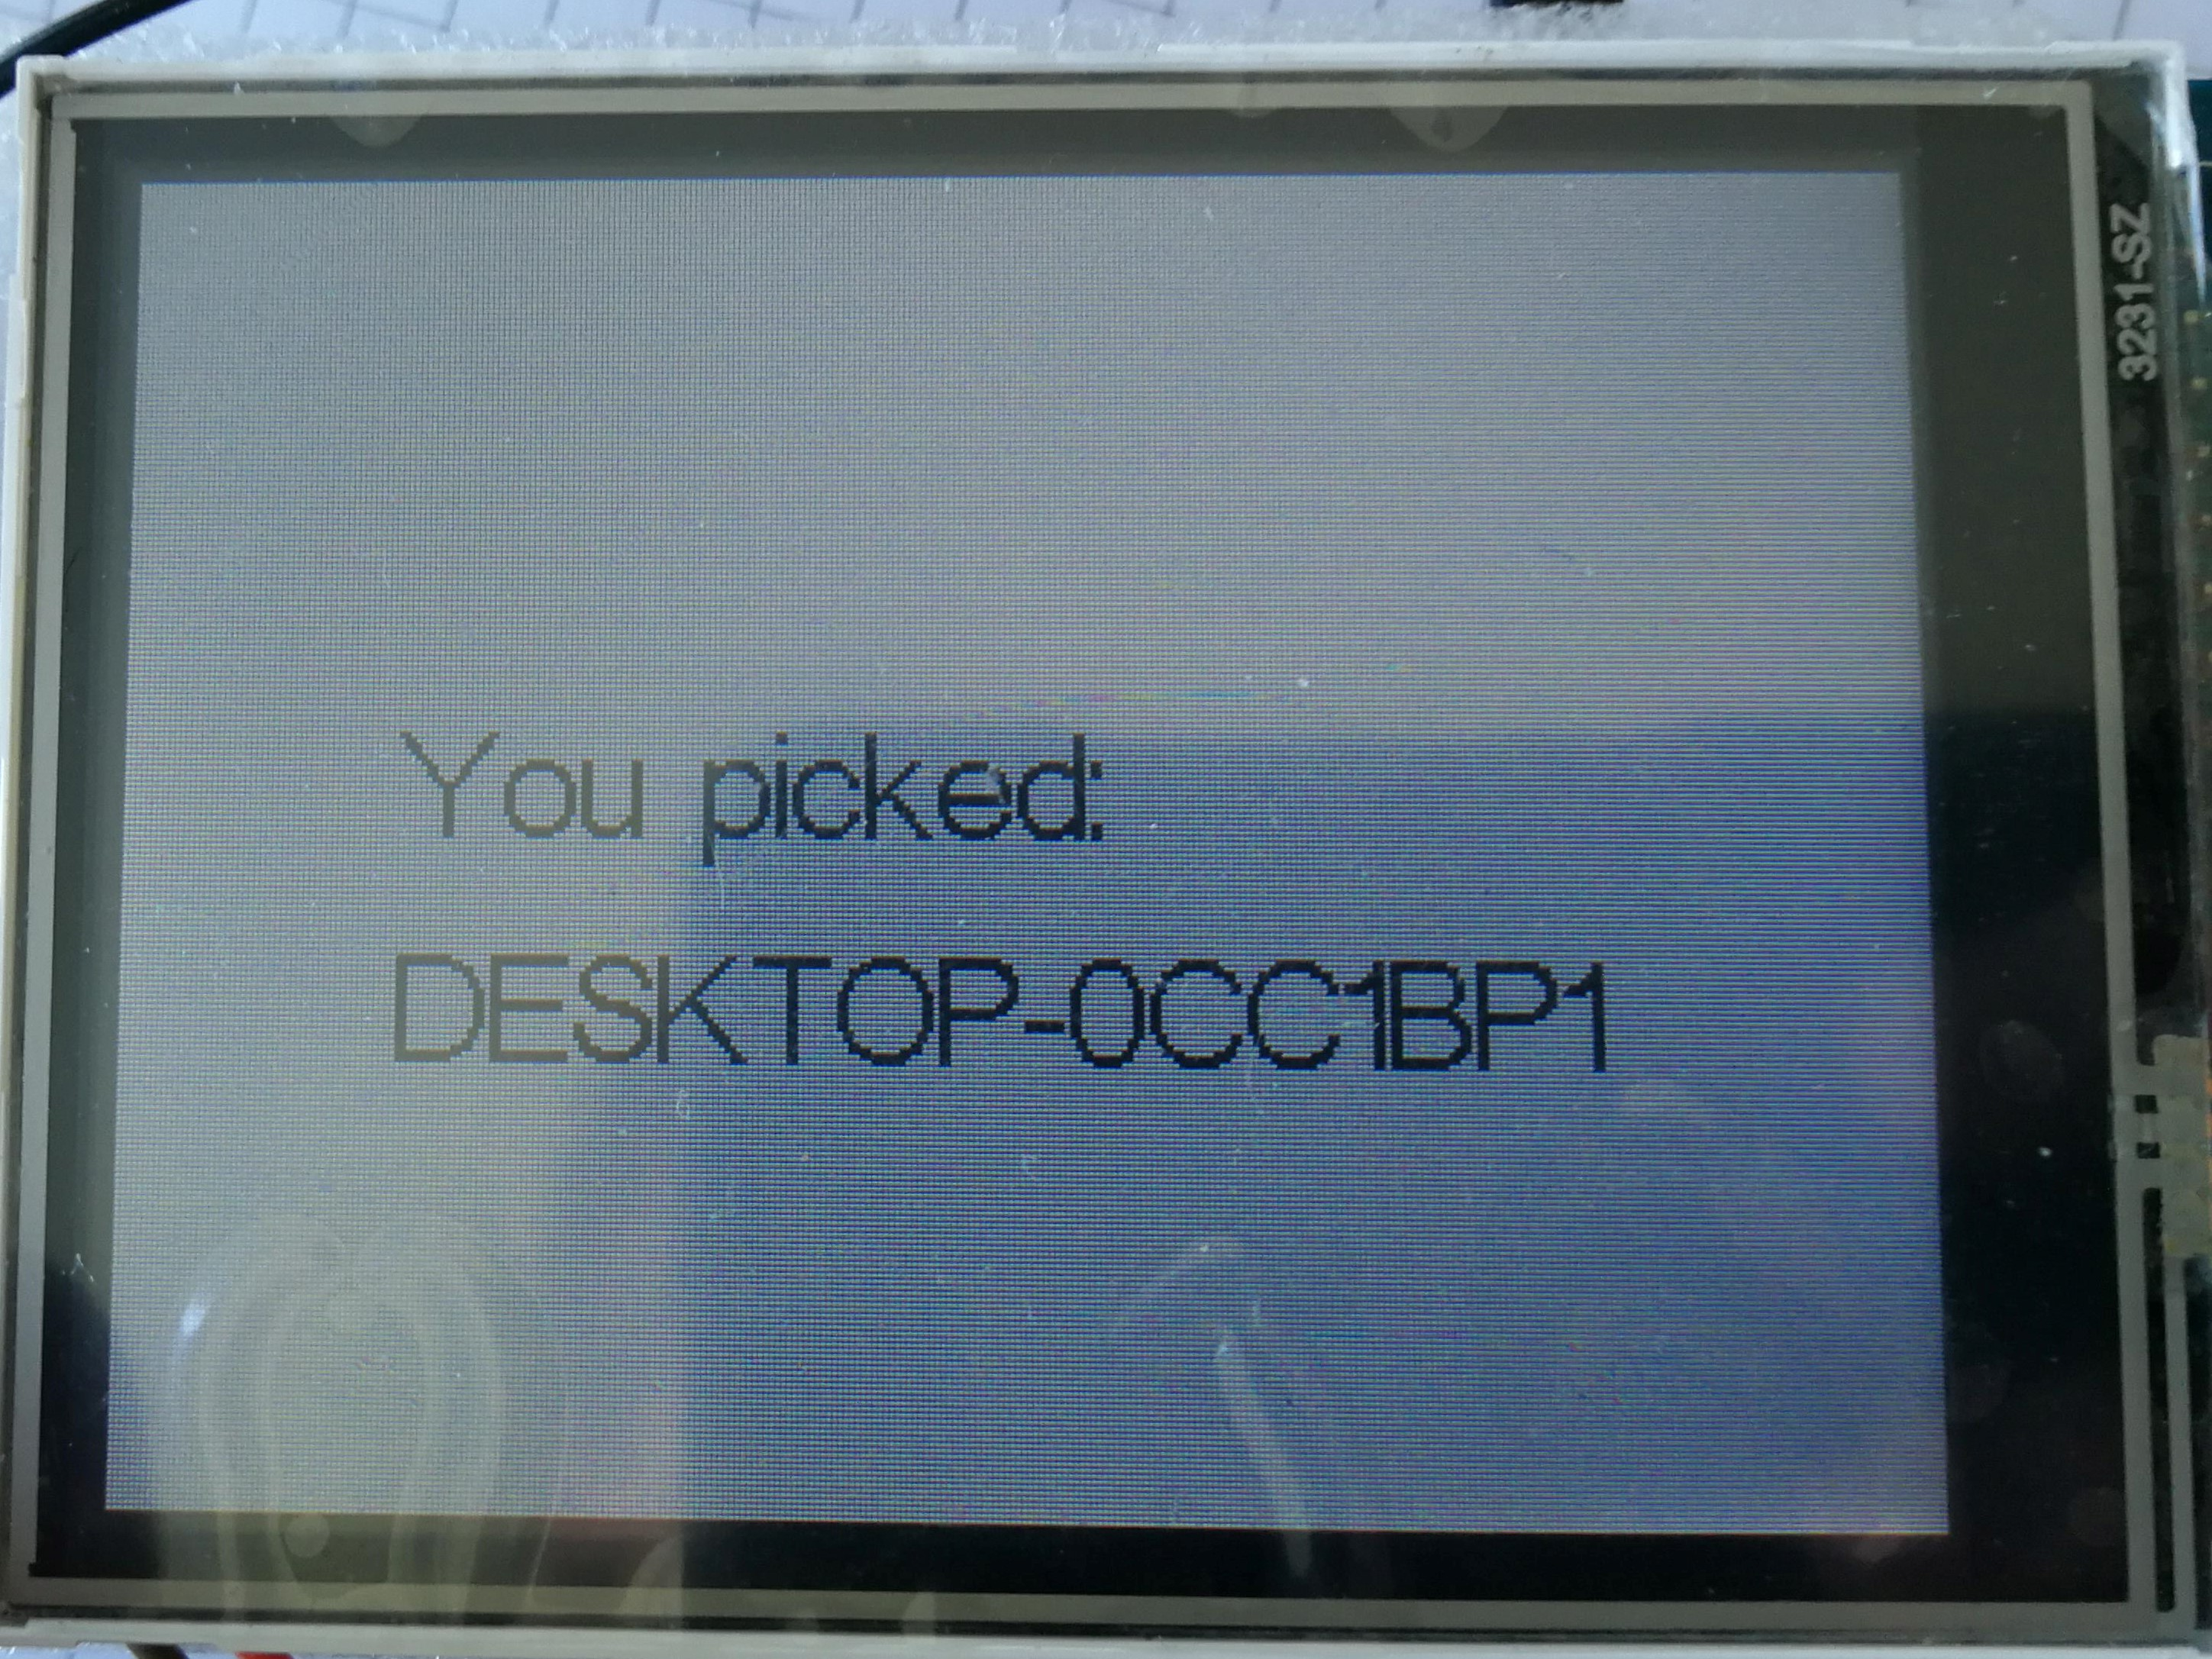
\includegraphics[width = 300 pt]{Img/pick.jpg}
	\caption{Brugergrænseflade: Valg af enhed}
	\label{fig:pick}
\end{figure}
Hvis brugeren herefter vælger funktionen "REMOVE DEVICE" fra figur \ref{fig:start}, åbnes der en liste over de godkendte Bluetooth-enheder der er gemt. Dette ses på figur \ref{fig:remove}. Hvis der på forhånd ikke er nogle gemte godkendte Bluetooth-enheder og listen dermed er tom, så vil displayet også være tomt, som vist på figur \ref{fig:noDevices}. 
\begin{figure}[H]
	\centering
	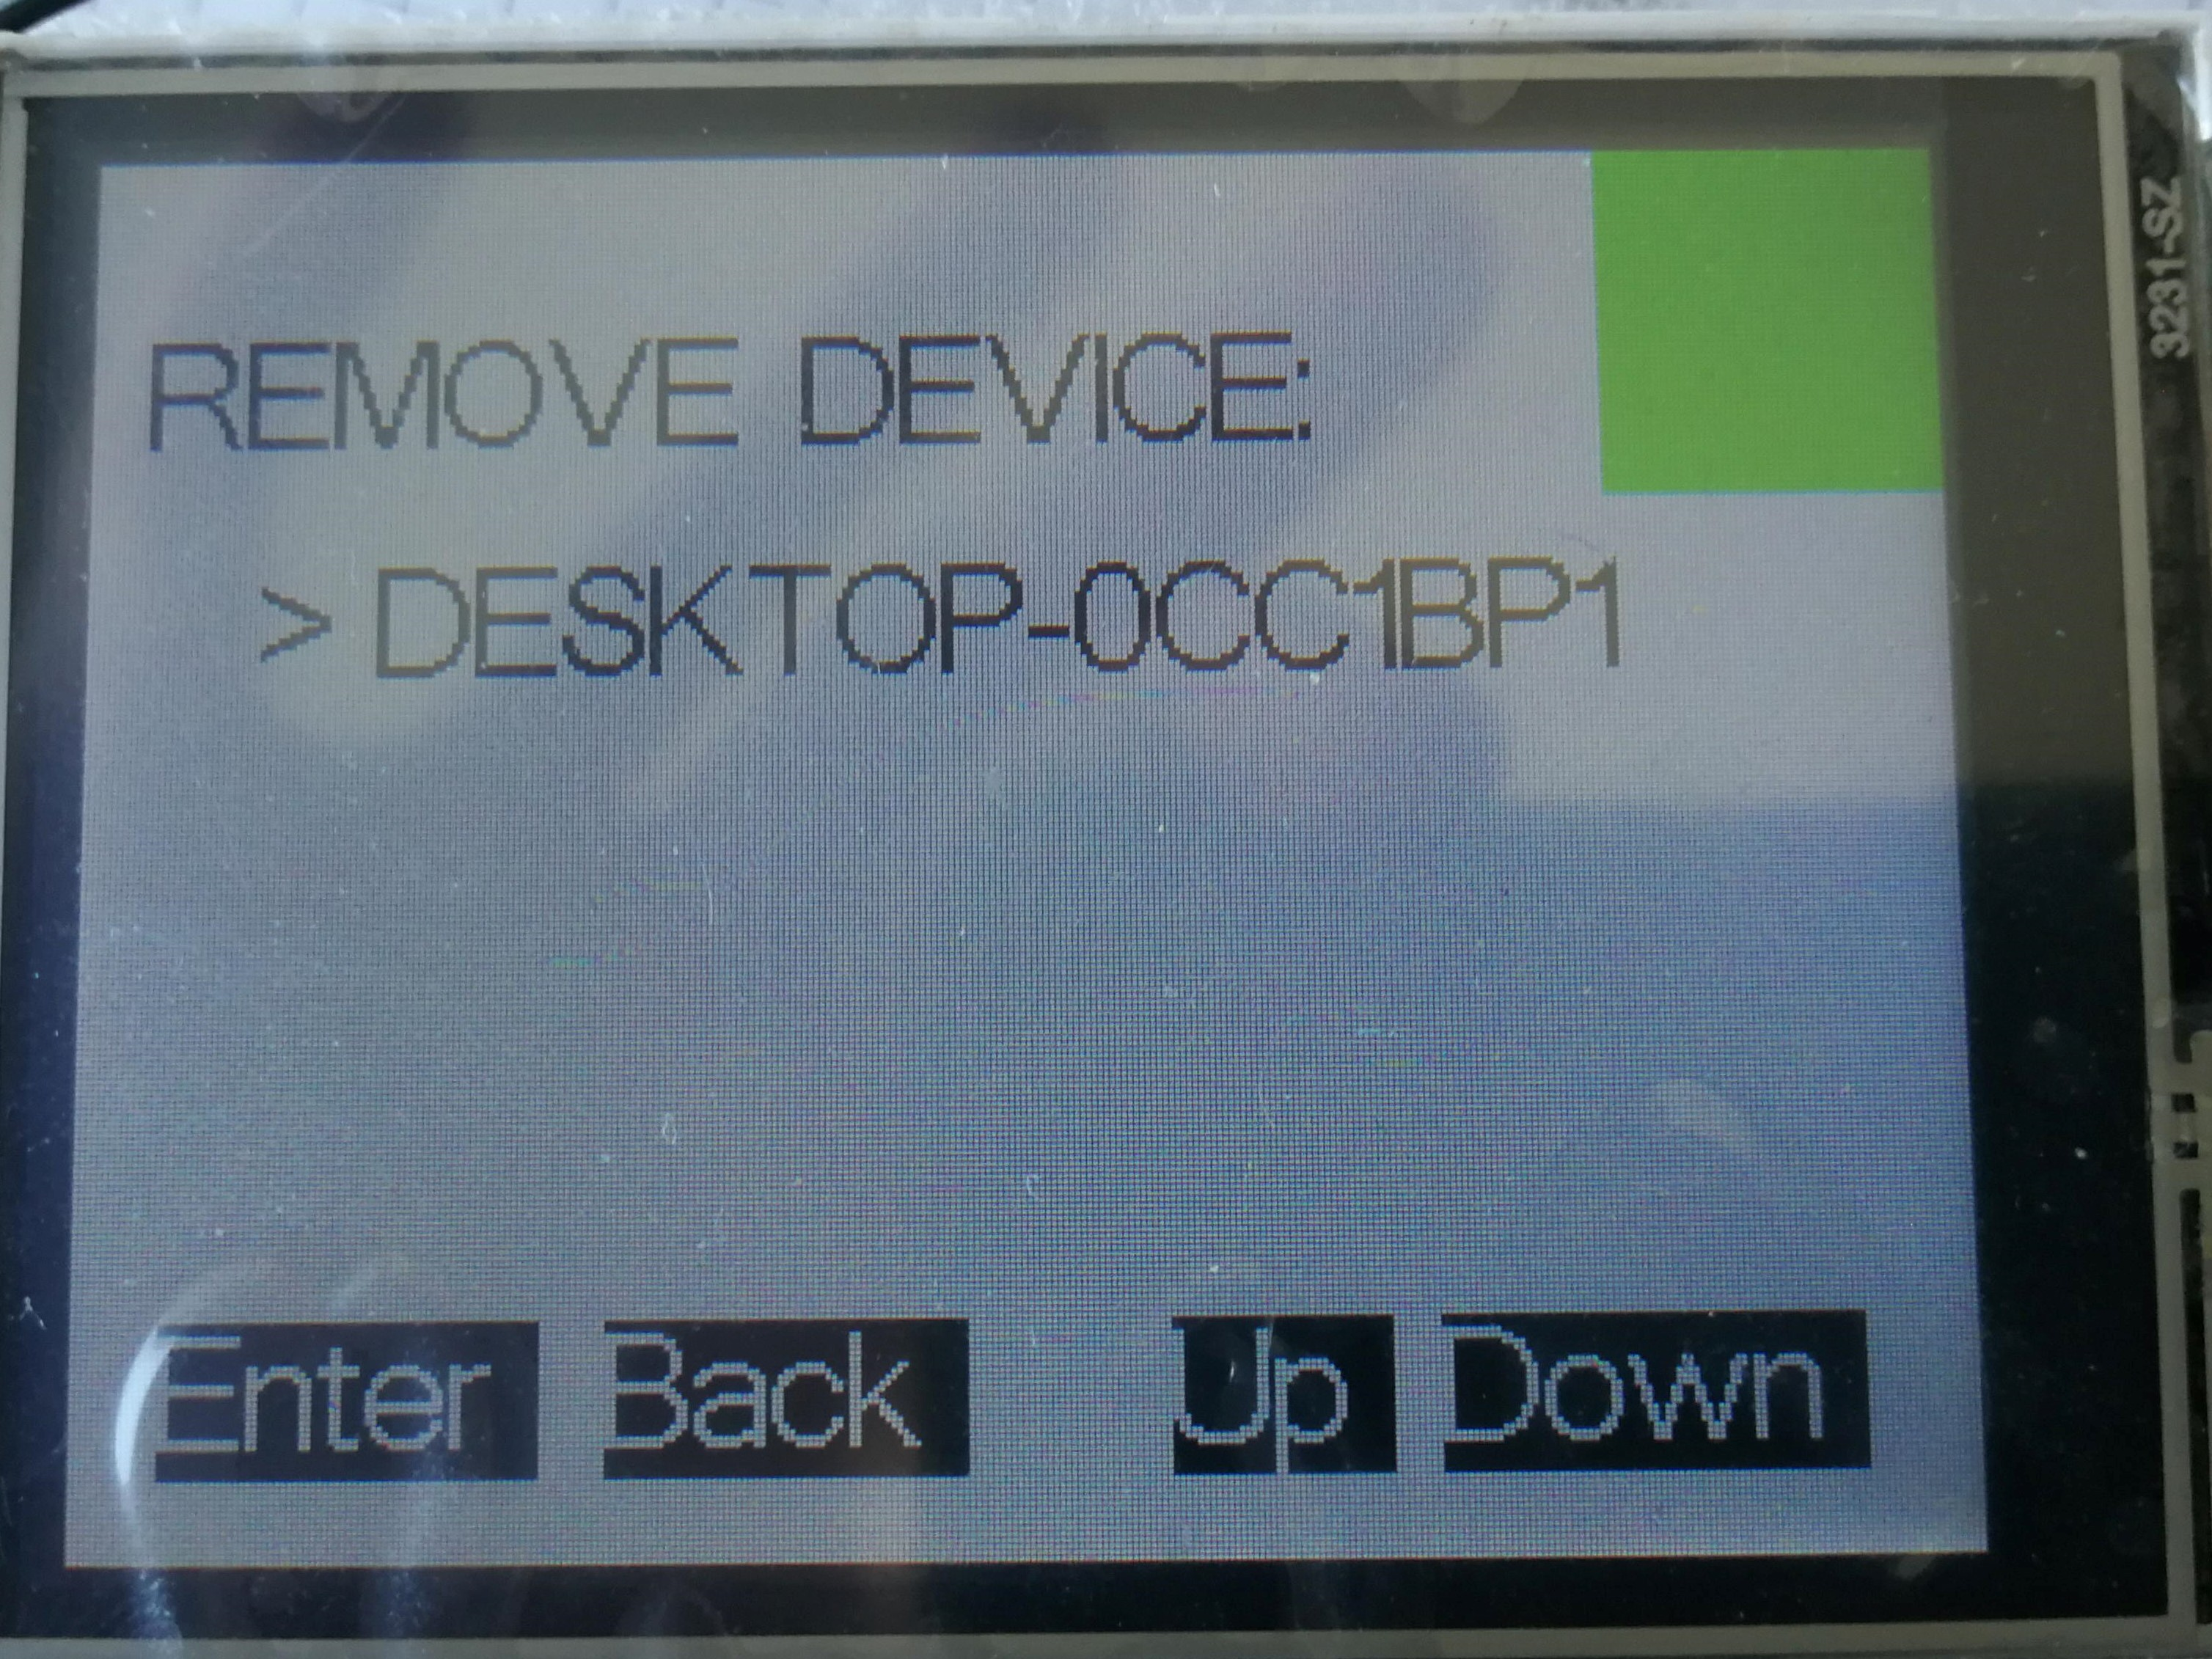
\includegraphics[width = 300 pt]{Img/remove.jpg}
	\caption{Brugergrænseflade: Fjern en enhed}
	\label{fig:remove}
\end{figure}
\begin{figure}[H]
	\centering
	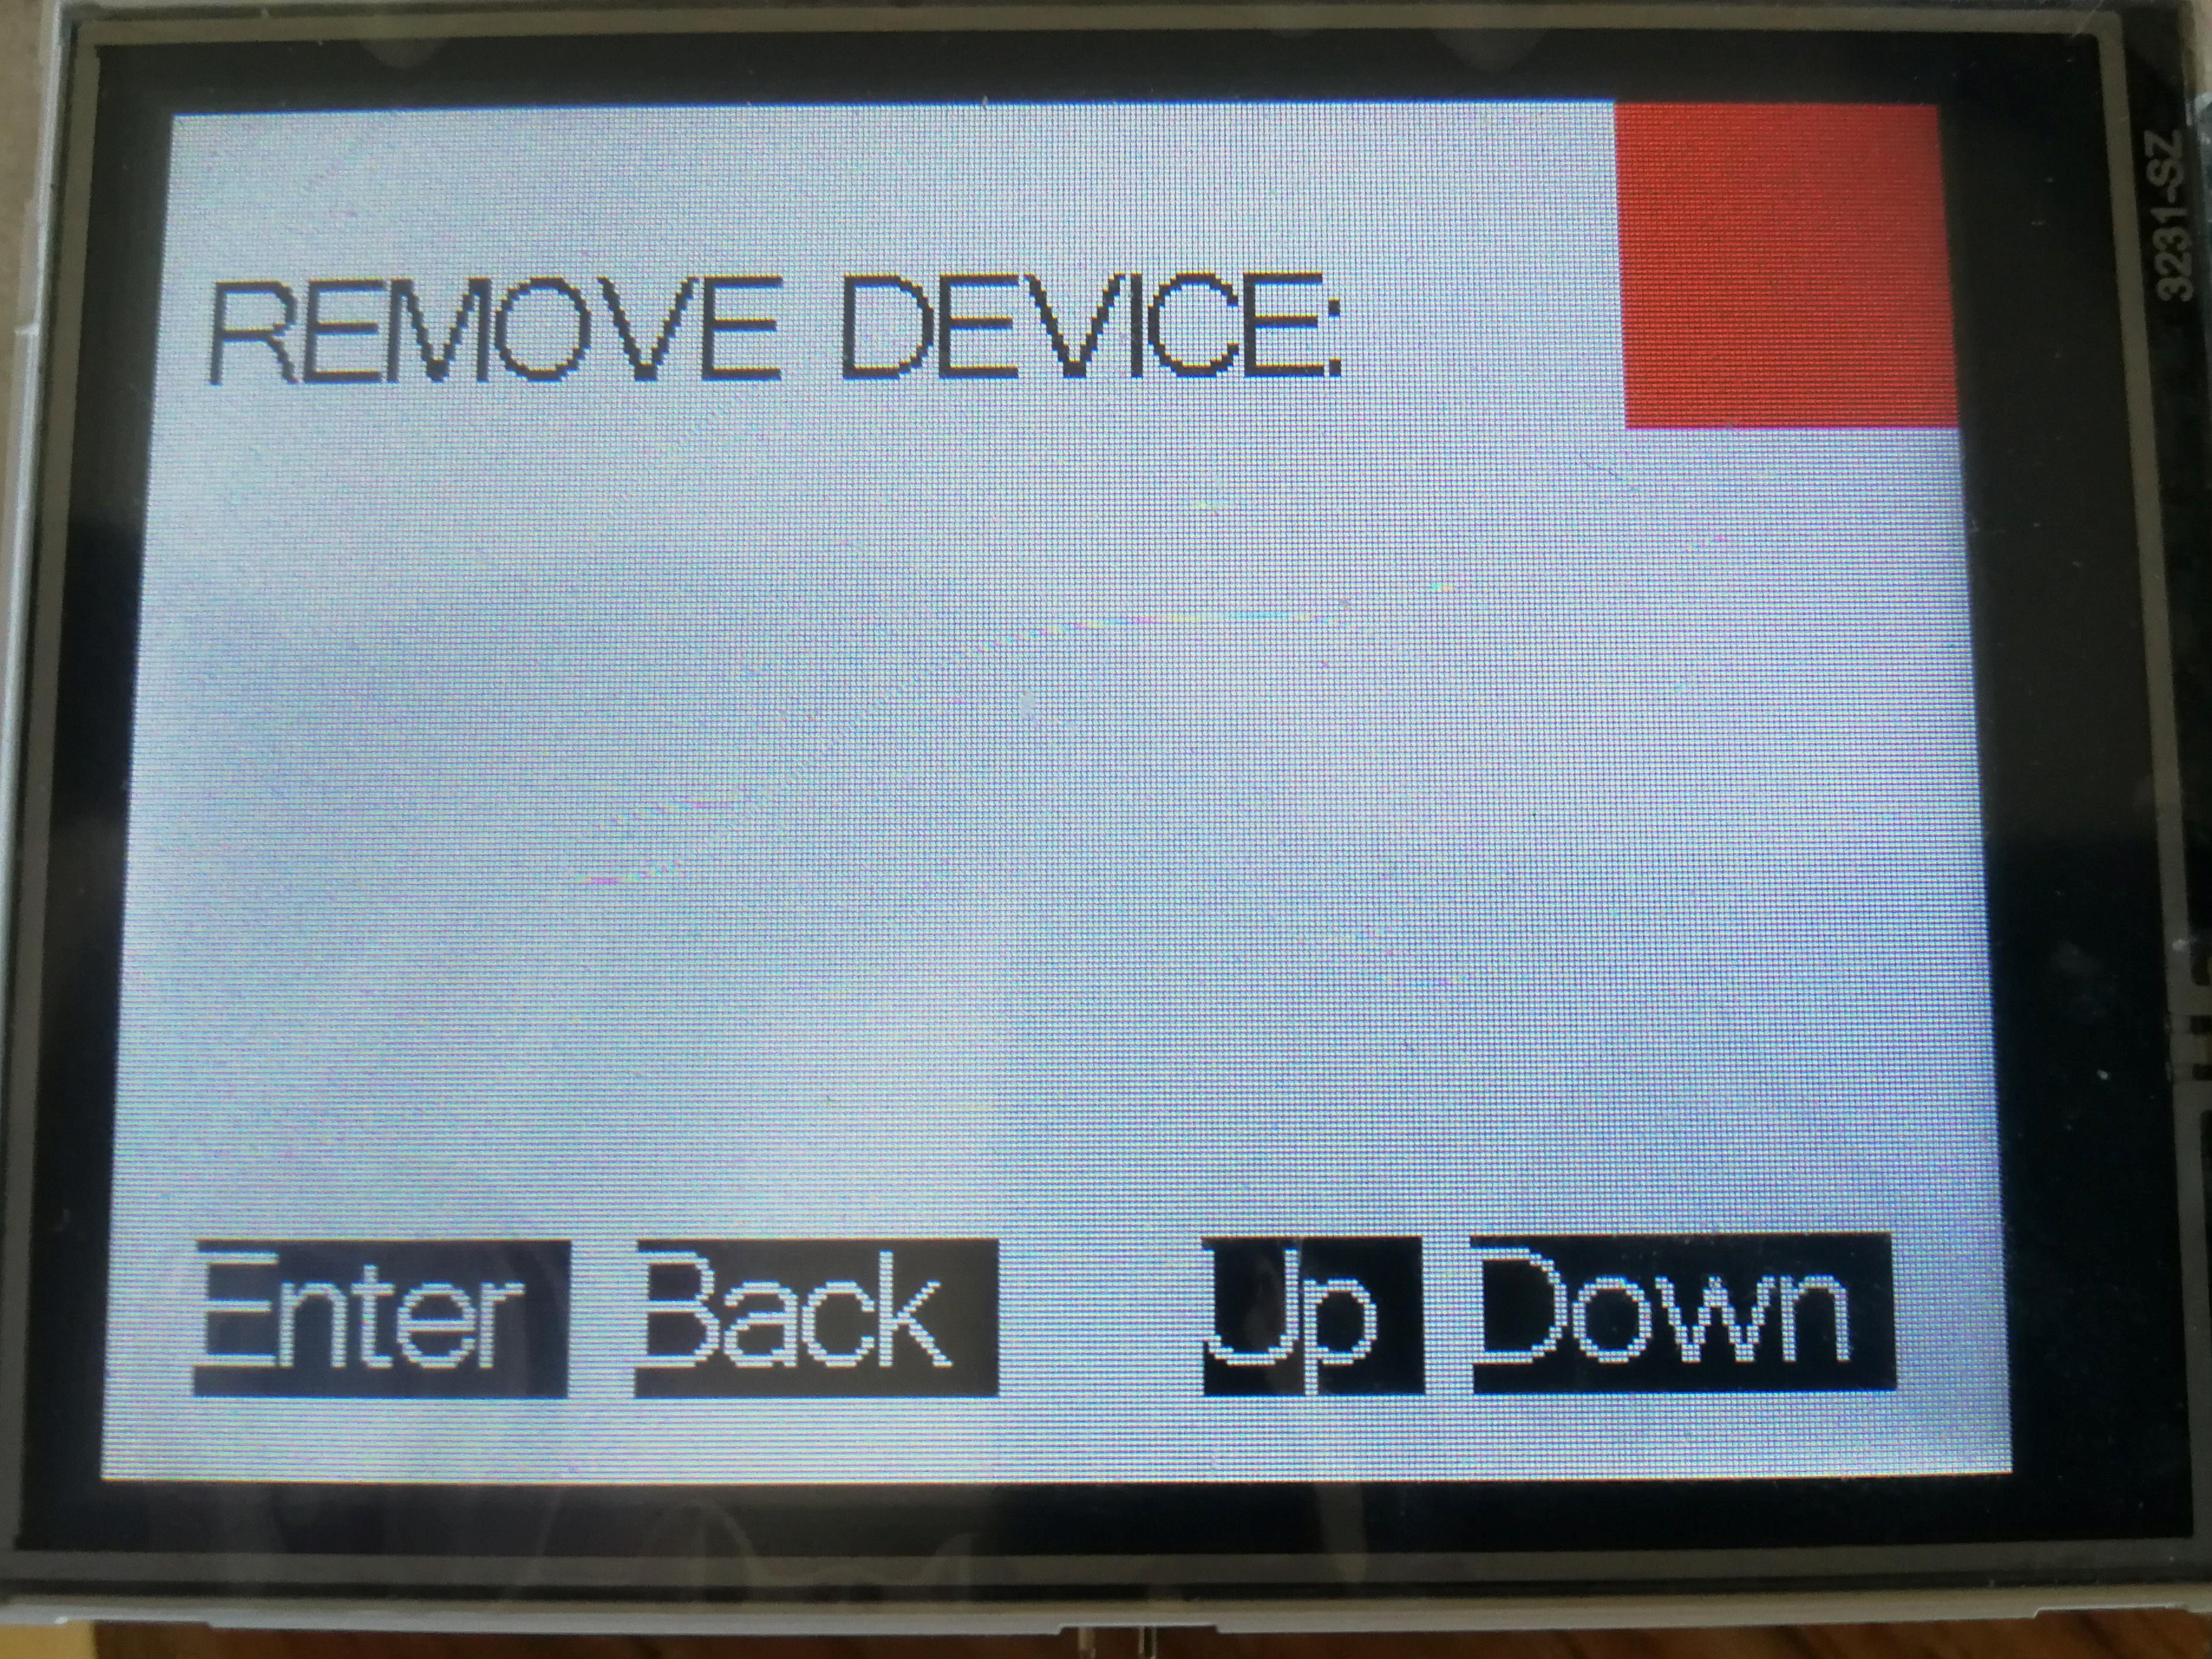
\includegraphics[width = 300 pt]{Img/noDevice.jpg}
	\caption{Brugergrænseflade: Ingen enehder}
	\label{fig:noDevices}
\end{figure}
Såfremt der er godkendte Bluetooth-enheder på listen, kan brugeren vælge at slette en bestemt enhed. Dette sker ved at trykke "Enter" ved enheden, som vælges ved hjælp af "Up" og "Down" og indikeres af pilen. Displayet viser på figur \ref{fig:delete} en besked om hvilken enhed brugeren har valgt at slette. 
\begin{figure}[H]
	\centering
	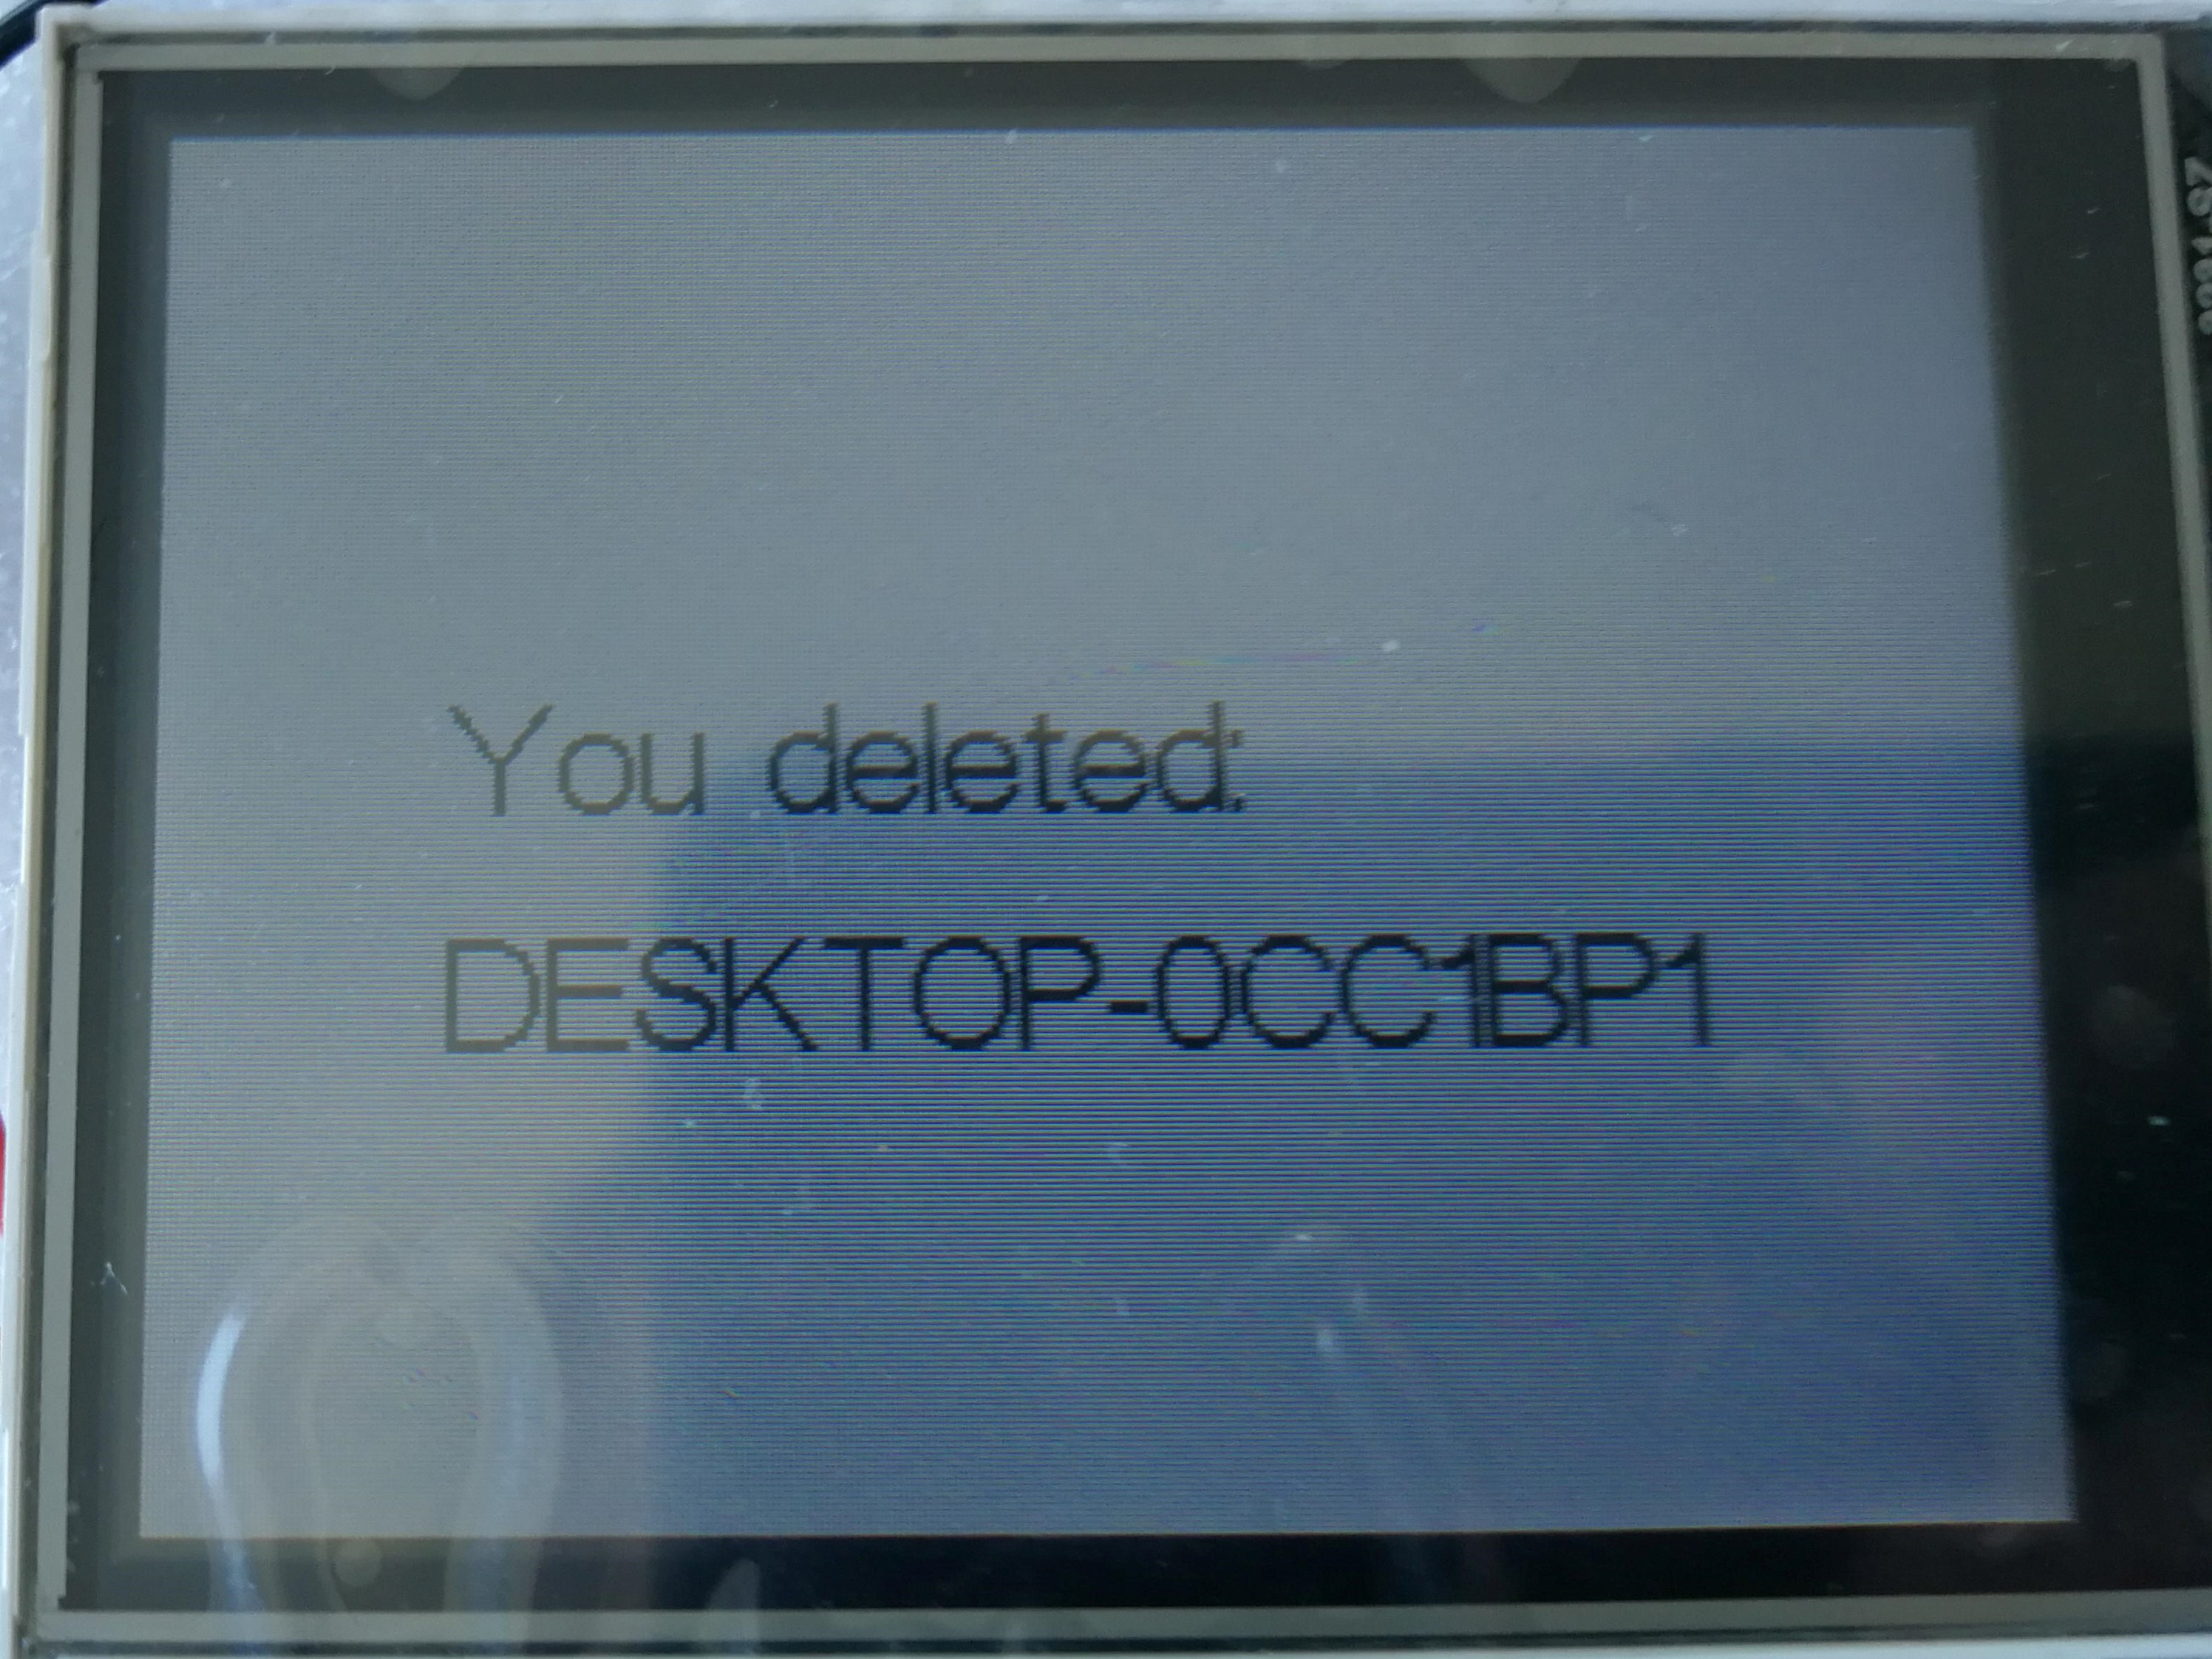
\includegraphics[width = 300 pt]{Img/delete.jpg}
	\caption{Brugergrænseflade: Valgt: fjernet en enhed}
	\label{fig:delete}
\end{figure}
Hvis brugeren vælger den sidste mulighed/state i hovedmenuen, "LOCK OFF", låses systemet op, teksten skifter og låsens indikator skifter farve. Dette ses på \ref{fig:lockOff}.
\begin{figure}[H]
	\centering
	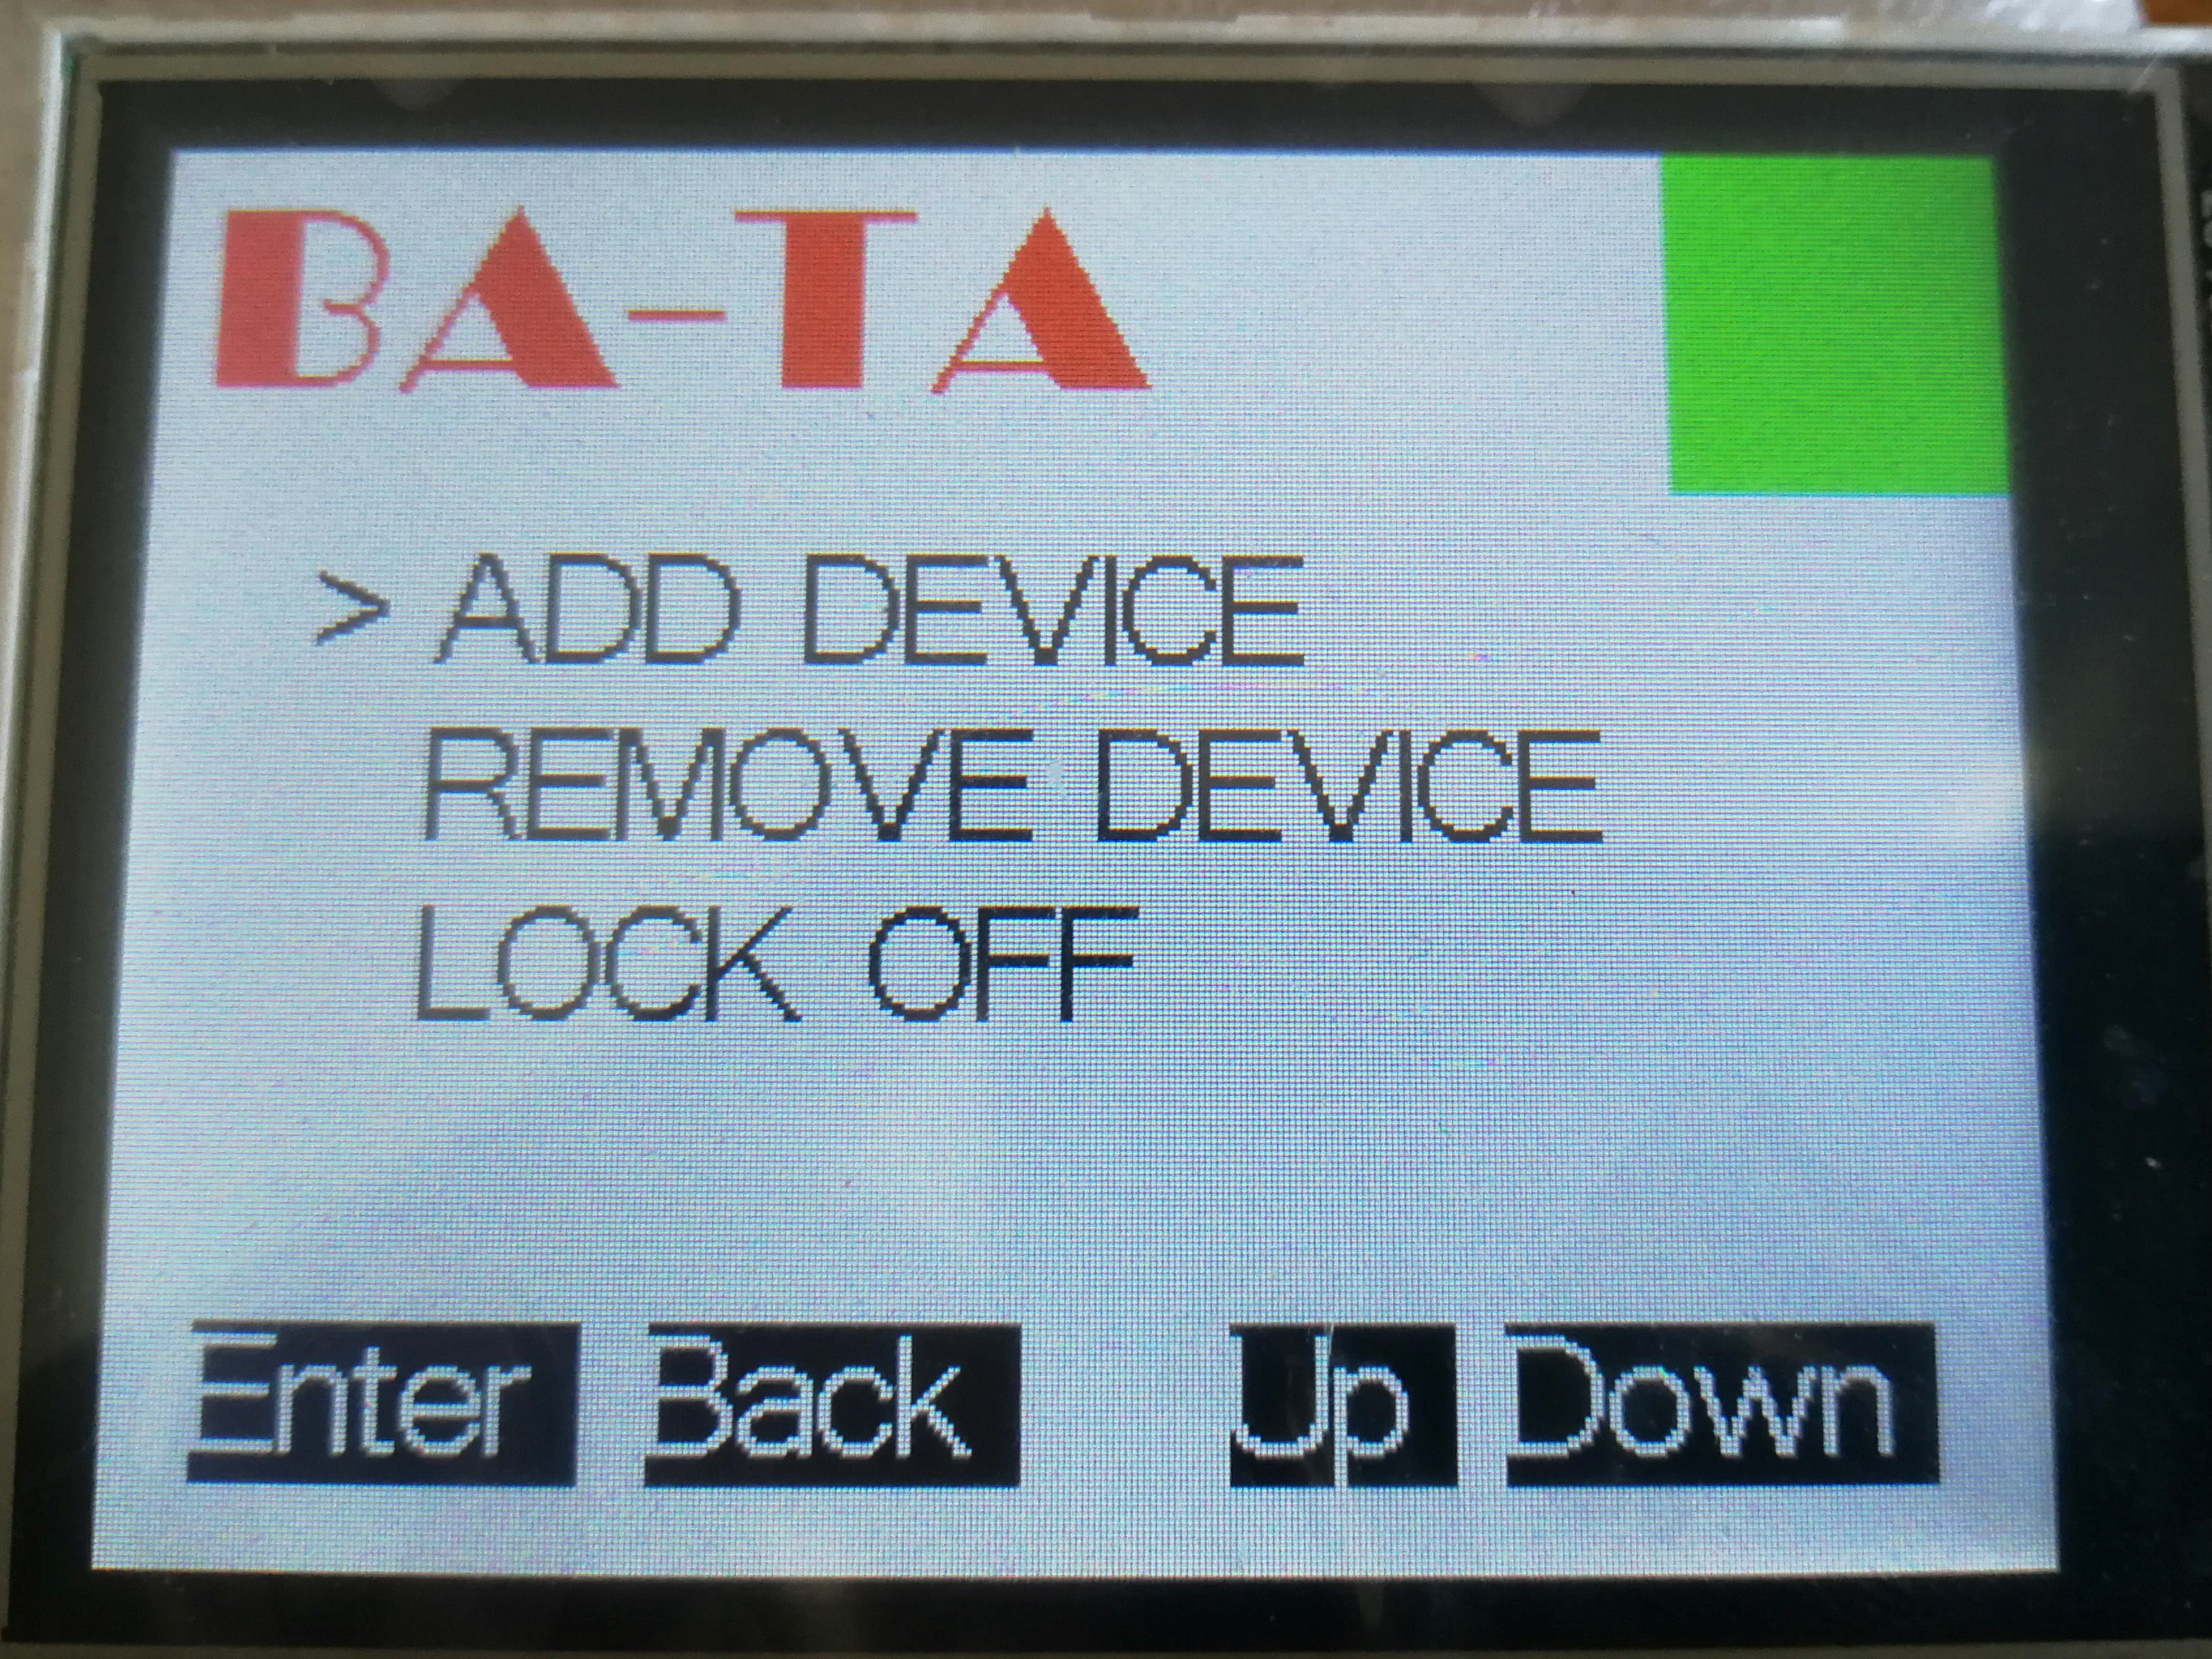
\includegraphics[width = 300 pt]{Img/lockOff.jpg}
	\caption{Brugergrænseflade: Låst op}
	\label{fig:lockOff}
\end{figure}
Hvis der endnu engang trykkes på den sidste state i hovedmenuen, ændres teksten, og låsen laver en "UPDATE"  hvert 5. sekund, og skifter låsen alt efter om der kan findes en Bluetooth-enhed, som også er på den godkendte liste. Dette ses på figur \ref{fig:auto}. Hvis der trykkes én gang til på sidste state, ændres låsens tilstand til at være manuelt låst.
\begin{figure}[H]
	\centering
	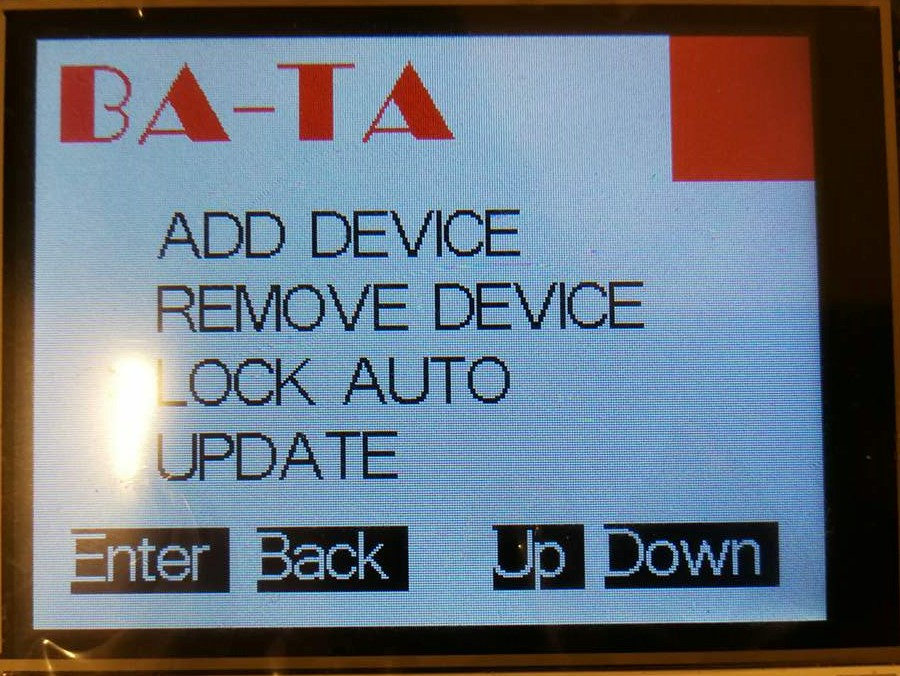
\includegraphics[width = 300 pt]{Img/auto.jpg}
	\caption{Brugergrænseflade: Lås Automatisk}
	\label{fig:auto}
\end{figure}


	%!TEX root = ../../Main.tex
\graphicspath{{Chapters/Drivers/}}
%-------------------------------------------------------------------------------


\section{Drivers}
I dette afsnit beskrives de forskellige drivere som er lavet til projektet. 
Driverne er delt op i flere forskellige cpp filer, dette er gjort for at gøre koden mere overskuelig, og gøre funktionaliteten mere effektiv. Herunder forsøges at gøre et overblik over de forskellige cpp filer og deres integeren.  


\subsection{Display driver}
Igennem øvelser til undervisningen, er der blevet opbygget en driver til et grafisk display. Igennem processen til dette projekt er der blevet modificeret og arbejdet videre på selvsamme driver. Cpp filen ligger under TFTdriver, som er bygget op af flere forskellige funktioner. I dette afsnit vil der gives et overblik over de mest essentielle funktioner. For at få en forståelse af selve opbygningen af driveren, henvises til datasheet for controlleren. 
\href{https://blackboard.au.dk/bbcswebdav/pid-1697983-dt-content-rid-3847230_1/courses/BB-Cou-UUVA-73302/BB-Cou-UUVA-65758_ImportedContent_20170106021228/BB-Cou-STADS-UUVA-52360_ImportedContent_20160107025559/LAB/Lab3a%20Graphic%20LCD%20Display/Files%20for%20LAB3a/ILI9341_v1.11.pdf}{ILI9341} \\
For at opbygge en basisforståelse for driveren, vil der først blive forklaret DisplayInit(). Først sætter vi de porte vi skal bruge fra Arduino til hhv. indgange og udgange. Vi har dog valgt ikke at have tilbagemeldinger, og derfor er der ikke initialiseret nogle indgange. Herefter sætter vi RESET, CS, WRX, RDX høje ift figur \ref{fig:Bus_timing}. Der bliver kørt en reset (tjek lige koden med timing, burde være kortere), for at resette displayet, og bagefter sendt fire kommandoer, som kan findes i command list i databladet. Sleep Out, Display On, Pixel format set = 16 bit og Memory Access Control (BGR = 1) (Tjek ift henning hvad dette gør). 



\begin{figure}[H]
	\centering
	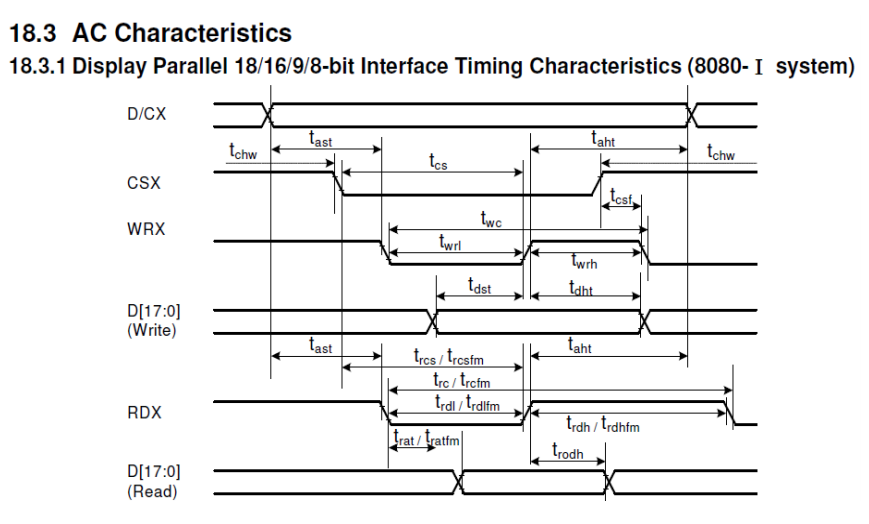
\includegraphics[width = 400 pt]{Img/Bus_timing.png}
	\caption{Bus Timing}
	\label{fig:Bus_timing}
\end{figure}

Herunder vil de essentielle funktioner deles op i hvert sin tabel. Flere af funktionerne gør brug af både Writecommand() og Writedata(), som er opbygget udfra Bus Timing figur \ref{fig:Bus_timing}. Derudover bruger flere af funktionerne SetColumnAddress() og SetPageAddress(), som er bygget op fra \href{https://blackboard.au.dk/bbcswebdav/pid-1697983-dt-content-rid-3847230_1/courses/BB-Cou-UUVA-73302/BB-Cou-UUVA-65758_ImportedContent_20170106021228/BB-Cou-STADS-UUVA-52360_ImportedContent_20160107025559/LAB/Lab3a%20Graphic%20LCD%20Display/Files%20for%20LAB3a/ILI9341_v1.11.pdf}{ILI9341} 
8.2.20. og 8.2.21.: \\
Nogle af funktionerne i driveren, bruges ikke i dette produkt, da flere af dem er brugt til test undervejs, for at kunne debugge den givne programstuktur.
\newline
\newline
\textbf{\large Included Font:}

\begin{center}
\begin{tabular}{ |l|l|l| }
\hline
\multicolumn{1}{ |c| }{\textbf{character.h}} \\
\hline
Karakter størrelse: 24*24 pixels  \\
Antal karakter: 95\\
\hline

\end{tabular}
\end{center} 
\begin{figure}[H]
	\centering
	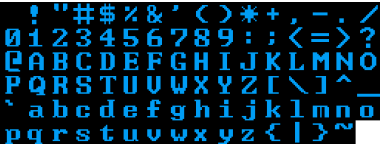
\includegraphics[width = 150 pt]{Img/Thedotfactory.png}
	\caption{The Dot Factory karakter}
	\label{fig:Thedotfactory}
\end{figure}

\textbf{\large Funktions:}

\begin{center}
\begin{tabular}{ |l|l|l| }
\hline
\multicolumn{1}{ |c| }{\textbf{ FillRectangle(StartX,StartY, Width, Height, Red, Green, Blue)}} \\
\hline
Funktion som laver en firkant med den valgte baggrundsfarve  \\
\hline
\textbf{Paramentre:}  \\ StartX: Startværdi på x-aksen \\StartY: Startværdi på y-aksen\\ Width: Bredden på firkanten\\ Height: Højde på firkanten\\ Red: farve(værdi)\\ Green: farve(værdi) \\ Blue: farve(værdi)\\
\hline
\end{tabular}
\end{center} 

FillRectangle er en funktion som visuelt kan ændre bits til en anden farve på den givne skærm. Fra input vælges startx og starty samt længde og bredde. Derefter laves en ud fra de input der er givet. Farven afhænger også af inputtet. Det der reelt sker, er at den givne farve bliver skrevet til hver eneste pixel, i det sted der er valgt en firkant. 

\begin{center}
\begin{tabular}{ |l|l|l| }
\hline
\multicolumn{1}{ |c| }{\textbf{ drawletters(str[],startx, starty,Red, Green, Blue)}} \\
\hline
Funktion som modtager en en streng, og konverterer ascii værdien til \\den rette værdi ift character.h \\
\hline
\textbf{Paramentre:}  \\str[]: Modtager en streng\\  Startx: Startværdi på x-aksen \\Starty: Startværdi på y-aksen\\ Red: farve(værdi)\\ Green: farve(værdi) \\ Blue: farve(værdi)\\
\\

\hline
\end{tabular}
\end{center}  

drawletters er en startfunktion til drawXletter, i denne funktion, findes længden på den på det givne tegn, som skal skrives. Herudover findes lægden at det givne loop drawXletter skal fortsætte, ift hvor mange bytes der hører til det givne tegn. Denne funktion står for at finde de respektive værdier fra array\_carrier, og sende dem med til drawXletter.  til sidst sættes den nye start\_x, hvor næste tegn kan placeres, her er der valgt et mellemrum fra udvikleren på 1 pixel.

\begin{center}
\begin{tabular}{ |l|l|l| }
\hline
\multicolumn{1}{ |c| }{\textbf{ drawXletter( bitmap[],length,count,startx,starty, letter, modulus,Red, Green, Blue)}} \\
\hline
Funktion som står for at skrive til hver bit, med værdier fra letterhelper()\\
\hline
\textbf{Paramentre:}  \\bitmap[]: Henter en byte fra character.h\\ length: Fortæller funktionen, hvor bred karakteren der skal skrives er\\ count: hvor mange bytes funktionen skal køre igennem for at lave hele karakteren\\ Startx: Startværdi på x-aksen \\Starty: Startværdi på y-aksen\\ Red: farve(værdi)\\ Green: farve(værdi) \\ Blue: farve(værdi)\\
\textbf{Note:} Funktionen sletter gamle karakterer, da en ny smallere karakter end forrige stadig\\ vil forblive på displayet\\

\hline
\end{tabular}
\end{center}  

drawXletters står for at farve hver pixel, så der laves det tegn som er anmodet, dette sker ved at funktionen modtager information fra drawletters, som har information om tegn[], som er hentet fra character.h. Dette array, består af et bitmap af alle ascii tegn, og byte værdier som tegner hver pixel. Igennem funktionen sikres at bredden på tegnet overholdes, og et nyt startx punkt bliver sat, samtidig med at starty (colum) sættes til næste linje. dette gøres indtil den del af arrayet er løbet igennem som er givet fra drawletters. Til sidst i koden slettes (pixels = hvid) tegn eller pixels, som ligger forand det nye tegn som er tegnet. Dette sker for at sikre at tegnene ikke flyder ind over hinanden, hvis der findes gamle tegn på pladsen, hvor den nye tegnes. 


\subsection{Touch driver}
Da projektet skulle bruge integering af en bruger, er der valgt at inkudere en touch driver som gør brug af \href{https://blackboard.au.dk/bbcswebdav/pid-1762166-dt-content-rid-4251461_1/courses/BB-Cou-UUVA-73302/BB-Cou-UUVA-65758_ImportedContent_20170106021228/BB-Cou-STADS-UUVA-52360_ImportedContent_20160107025559/LAB/LAB10%20Touch%20Screen%20Driver/Files%20for%20LAB10/XPT2046.pdf}{XPT2046}
Touch Screen Controller, som allerede var en del af \href{https://blackboard.au.dk/bbcswebdav/pid-1762173-dt-content-rid-4251448_1/courses/BB-Cou-UUVA-73302/BB-Cou-UUVA-65758_ImportedContent_20170106021228/BB-Cou-STADS-UUVA-52360_ImportedContent_20160107025559/LAB/LAB10%20Touch%20Screen%20Driver/Files%20for%20LAB10/DS_IM120417024_ITDB02ArduinoMEGAShield.pdf}{ITDB02}
Arduino MEGA shield, som bliver også bliver brugt i Display driveren. \\
Driveren har tre funktioner, hvor Init() sætter de forskellige porte til hhv indgange og udgange, og derefter sætter de respektive ben til enten høj og lav. Funktionen pulse() står for at lave en puls på clk benet som er opsat ift. Figur 15 i \href{https://blackboard.au.dk/bbcswebdav/pid-1762166-dt-content-rid-4251461_1/courses/BB-Cou-UUVA-73302/BB-Cou-UUVA-65758_ImportedContent_20170106021228/BB-Cou-STADS-UUVA-52360_ImportedContent_20160107025559/LAB/LAB10%20Touch%20Screen%20Driver/Files%20for%20LAB10/XPT2046.pdf}{XPT2046}
datasheet. 
Herunder vil der laves en tabel over den sidste funktion. 

\begin{center}
\begin{tabular}{ |l|l|l| }
\hline
\multicolumn{1}{ |c| }{\textbf{TouchRead(xy)}} \\
\hline
Funktion som står for at læse værdien fra brugerinputtet.\\
\hline
\textbf{Paramentre:}  \\ xy: Styrer om retur værdien skal være for x eller y \\
\textbf{Retur:} Værdien for enten x eller y. \\
\\

\hline
\end{tabular}
\end{center}  

TouchRead står for at læse den værdi som bliver sendt over en seriel linje fra touch controlleren. Denne værdi skal ligges korrekt ind i en int, og bliver lagt en til hver bit, hvor gang der modtages ettal på PINE bit 5, herefter retuneres int værdien. 


\subsection{Bluetooth modul}

Bluetooth-modulet der bliver brugt i BA-TA systemet er af typen HC-05. Denne type-version understøtter nemlig mulighed for at tage rollen som både Master/Slave i et Bluetooth Master/Slave forhold imellem to parrende Bluetooth-enheden. Bluetooth modulet er sammensat med et breakout- board i bunden af modulet, hvilket giver nem adgang til de brugbare pins på selve Bluetooth-modulet, hvilket også kan ses på figur \ref{fig:bluetooth_modul}

\begin{figure}[H]
	\centering
	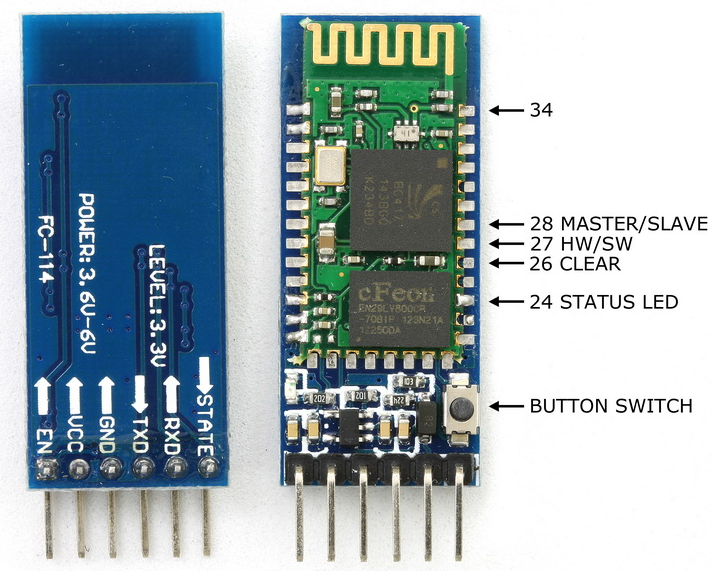
\includegraphics[width = 200 pt]{Img/modul.PNG}
	\caption{Bluetooth modulet: HC-05 GW-040.}
	\label{fig:bluetooth_modul}
\end{figure}

\subsubsection{Protokol}
Der kommunikeres til systemets Bluetooth-modul igennem en UART-forbindelse. Gruppens implementerede UART-driver på Arduino’en gør det muligt, at Arduinoen og Bluetooth-modulet kan kommunikere sammen vha. AT-kommandoer. 
AT-kommandoerne (Attention-commands) som Bluetooth-modulet understøtter kan bruges til generel opsætning af modulet, sætte Master/Slave roller, scanne for nærtliggende Bluetooth-enheder, samt at spørge om navn på fundne Bluetooth-enheders adresser. AT-kommandoerne er en general standard som bruges til at sende instruktioner til et modul og dermed er de opbygget på samme måde for hvert modul der bruger dem. På en etableret UART forbindelse vil man kunne sende en ”AT+kommando” til modulet, hvorefter modulet vil udføre kommandoen, og evt sende et svar tilbage, samt et OK, hvilket indikerer at beskeder var succesfuldt modtaget af modulet. Det samme er gældende for HC-05 Bluetooth modulet som indgår i BA-TA systemet.
Eksempler på brugte AT-kommandoer til Bluetooth-modulet i BA-TA:

\begin{itemize}
	\item ”AT+INIT” – Initialisering af Bluetooth-modulets Bluetooth SPP profil
	\item “AT+INQM,0,5,4” – Sætter scanner parameter. I dette tilfælde at der maksimum skal findes 5 Bluetooth enheder og at timeout på en scanning af Bluetooth enheder er 4*1.28 sekunder.
	\item ”AT+RNAME?<indsæt,Adresse,Her>” – Bluetooth-modulet spørger om navnet på adressen til den respektive indsætte adresse.
\end{itemize}

En succesfuld AT-kommando vil altid få Bluetooth-modulet til at returnere et OK. Såfremt der eksempelvis bliver spurgt om et navn på en respektiv Bluetooth-enheds adresse, så vil Bluetooth-modulet også returnere den fundne Bluetooth-enheds navn og et OK til sidst. 

\begin{figure}[H]
	\centering
	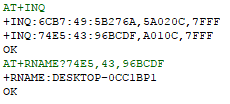
\includegraphics[width = 200 pt]{Img/uart_eksempel.PNG}
	\caption{Kommunikationseksempel med AT-kommandoer ved brug af en UART forbindelse til Bluetooth modulet.}
	\label{fig:UART_eksempel}
\end{figure}

På ovenstående figur,  \ref{fig:UART_eksempel}, kan vi se et eksempel på kommunikation vha. en UART forbindelse til Bluetooth modulet. I eksemplet bliver der sendt et "AT+INQ" til Bluetooth-modulet. Denne besked betyder inquiry, og derfor går Bluetooth modulet straks igang med at undersøge hvilke nærtliggende Bluetooth enheder den kan finde. Herefter svarer den tilbage med et "+INQ:<AdressePåFundetEnhed>" hver gang den har fundet en ny enhed. Dette forsætter den med indtil den når sit maks antal devices eller timeout grænse, som er bestemt af kommandoen "AT+INQM". Når timeout eller maks antal enheder er nået returnerer Bluetooth modulet også et OK for at indikere at den er færdig. Herefter er den også klar igen til at modtage nye beskeder.

\subsubsection{Implementering}

Da AT-kommandoerne og retur-beskederne er opbygget med samme struktur, har gruppen med fordel taget brug af dette til, at kunne udvikle en Bluetooth-kommunikations-driver, som netop udnytter denne gentagende og genkendelige proces. 

\begin{figure}[H]
	\centering
	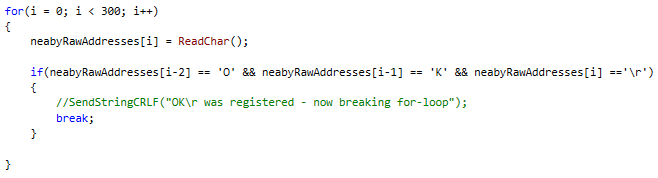
\includegraphics[width = 400 pt]{Img/OK_registrered.PNG}
	\caption{Registrering af det returnede "OK" fra Bluetooth modulet}
	\label{fig:OK_registrered}
\end{figure}

På figur \ref{fig:OK_registrered} kan vi se et eksempel på, hvordan gruppen har udnyttet at der altid vil blive sendt et OK retur til sidst, når Bluetooth modulet indikerer at den er færdig med den instruktionen/kommandoen som den har modtaget forinden. I eksemplet fra figuren benytter gruppen sig af dette til at tjekke hvornår Bluetooth modulet har sendt alt information om Bluetooth enheders adresser, som den har registreret ved sit "AT+INQ".

\begin{figure}[H]
	\centering
	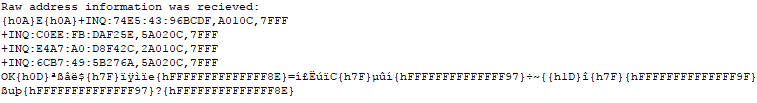
\includegraphics[width = 500 pt]{Img/raw_address.PNG}
	\caption{Al rå adresse information modtaget fra Bluetooth modulet}
	\label{fig:raw_address}
\end{figure}

Herefter kan der analyseres på det char array som alt adresse information for alle fundne enheder ligger i. Formålet med dette er at få skilt informationen ad således vi tage separere de forskellige adresser fra hinanden. Dette skyldes at dataen i det pågældende char array højst sandsynligt er loaded med flere adresser, som det eksempelvis kan ses på figur \ref{fig:raw_address}

Næste skridt er hermed at skille alt den information vi får udover MAC-adressen til de bestemte enheder. Dette gøres ved brug af "delimeter" princippet. Delimeter princippet kan bruges i dette tilfælde, da alle modtagede adresser i char array'et er sammensat og seperaret fra hinanden på en kontinuerlig måde. Hver MAC-adresse starter efter "+INQ:, de 3 dele af MAC adressen er separeret af ":" og MAC-adressen slutter ved et ",". Dette kan også ses på figur \ref{fig:raw_address}.


\begin{figure}[H]
	\centering
	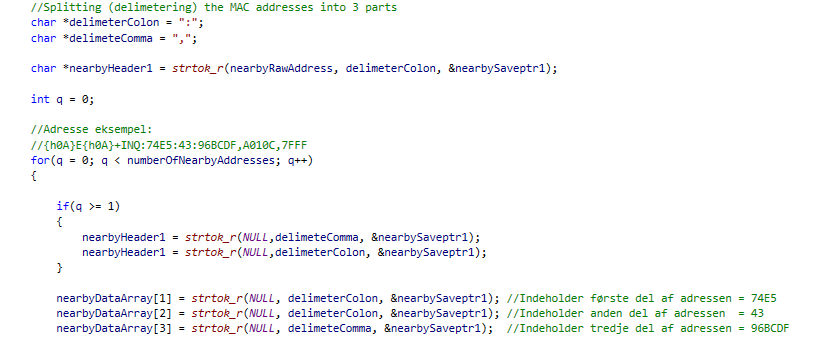
\includegraphics[width = 500 pt]{Img/delimetering.PNG}
	\caption{Brug af "delimeter"\-princippet ved brug af strtok\_r funktionen}
	\label{fig:delimeter}
\end{figure}

På ovenstående figur, \ref{fig:delimeter}, kan vi se det "delimeter"-princippet som er taget i brug for at kunne skære alt andet end de 3 dele af adressen (i dette tilfælde, 74E5, 43 og 96BCDF).

Herefter skal addressen nemlig sammensættes på en ny måde, således at vi kan få Bluetooth modulet til at spørge adressens respektive Bluetooth enhed om enhedens navn. Dette er en nødvendighed for at kunne vise navnet til brugeren i brugergrænsefladen i use case 1 og use case 2.

Før at Bluetooth modulet kan registrere at systemet forespørger navnet på en fundet Bluetooth enhed, og dens respektive adresse, skal det dermed følge denne form:\\ "AT+RNAME?74E5,43,96BCDF" og ikke:\\ "AT+RNAME?74E5:43:96BCDF", som vi modtog adressen i første omgang fra Bluetooth modulet. Forskellen er ikke stor, men udbytningen af koloner til kommaer er forskellen på om Bluetooth modulet kan genkende og eksekvere kommandoen den modtager. Dermed har der været et implementeringsbehov for at kunne tage højde for dette. Dette tager resten af koden i funktionerne addressDelimeter og trustedAddressDelimeter sig af. Forskellen på disse to funktioner er at den ene bruges til at gøre det for de enheder som skal på den godkendte liste over Bluetooth enheder i systemet. addressDelimeter bruges derimod til når låse staten er sat til auto, da funktionaliteten i de 2 funktioner varierer i forhold til hinanden.

\textbf{*** HVIS DER ER PLADS TIL MERE TEKST KAN NAVNE-FUNKTIONEN GODT UDDYBES HER}

\subsection{SystemMaster}
Dette driver/modul, står for at forbinde de andre cpp filer, og for at køre systemets funktionalitet. Derfor kaldes denne klasse også for master, da den fungerer som master ift. de andre klasser, som derved er slaves. Ift figur \ref{fig:Entity}, ses Touch.h ikke som implementeret i denne klasse. Dette skulle den have været, men pga tidspres blev dette nedprioteret, derudover skulle klassen counting\_millis.c også være implementeret, mere om det i afsnittet Tekniske overvejelse og valg. 
Heruder vil kort gives et overblik over koden:
\newline
\newline
Strukturen i koden er bygget op af forksellige states, som systemet kan komme i. I hver state, bruges flere forskellige funktioner, for at skabe det display som vist i afsnittet Brugergrænseflade. På figur \ref{fig:dafaultkode} vises
et udklip fra dafault staten, som laver Hoved Menuen fra afsnittet Brugergrænseflade. 
\begin{figure}[H]
	\centering
	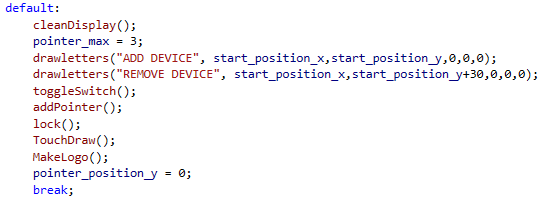
\includegraphics[width = 300 pt]{Img/dafaultkode.PNG}
	\caption{Koden til default staten}
	\label{fig:dafaultkode}
\end{figure}

Funktionaliteten fungerer på den måde at hvis auto mode sat i Hoved Menuen, vil der tjekkes for gemte enheder ift nye adresser som modtages fra bluetooth modulet. Det forløbige produkt, har en update state, som vises når den opdaterer nye værdier, og derved ikke kan brugeren ikke integere med systemet samtidig. Dette kan ses på figur \ref{fig:auto}
	%!TEX root = ../../Main.tex
\graphicspath{{Chapters/Alternative/}}
%-------------------------------------------------------------------------------


\section{Tekniske overvejelse og valg}


Da projektets omfang og opbygning har været meget frit, er der også blevet lavet nogle valgt og fravalg i process fasen. Dette vil vi give et overblik over i dette afsnit, forklare fordele og ulmeper ved hvert modul vi har valgt, og driverne dertil. Herunder gives et overblik over de emner gruppen mener har været mest essentielle ift fordele og ulemper af de forekellige moduler. 

\subsection{TFT Display} 
Da omfanget for projektet inkluderede et display, gjorde gruppen et valg om at bruge TJC-9341-032 som display, og \href{https://blackboard.au.dk/bbcswebdav/pid-1697983-dt-content-rid-3847230_1/courses/BB-Cou-UUVA-73302/BB-Cou-UUVA-65758_ImportedContent_20170106021228/BB-Cou-STADS-UUVA-52360_ImportedContent_20160107025559/LAB/Lab3a%20Graphic%20LCD%20Display/Files%20for%20LAB3a/ILI9341_v1.11.pdf}{ILI9341} 
som display controller. Dette \href{https://blackboard.au.dk/bbcswebdav/pid-1697983-dt-content-rid-3847230_1/courses/BB-Cou-UUVA-73302/BB-Cou-UUVA-65758_ImportedContent_20170106021228/BB-Cou-STADS-UUVA-52360_ImportedContent_20160107025559/LAB/Lab3a%20Graphic%20LCD%20Display/Files%20for%20LAB3a/ILI9341_v1.11.pdf}{ILI9341} 
er valgt på baggrund af, gruppen har abejdet med dette display modul tidligere, derudover var dette også tilgængeligt.
Til selve display'et er der valgt kun at kunne skrive til display'et og ikke læse fra det. Fordelen ved kun at sende data til displayet, er at det gør opsætningen meget nemmere for udvikleren. \\
Fordelen ved at intialisere driveren til at kunne modtage data fra displayet, ville være at programstrukturen, kunne spørge skærmen hvilket display, der var på skærmen nu. Dette vil sikre at programstrukturen altid ved hvilket frame der vises på displayet. Ulempen ved den måde gruppen har intialiseret driveren på, er at microcontroller skal holde styr på hvilken frame, der vises på skærmen. Dette gør det mere udfordrende for udvikleren, og derved gør at koden kommer til at fylde mere. Hvis driveren skulle laves på en memory kritisk microcontroller, ville det være en fordel at tilføje skærmen at kunne læse hvilket frame der står på skærmen. \\
Vi har ikke brugt meget tid på at undersøge alternative display. Der blev valgt at et Alphanumeric display, som tidligere var bearbejdet, ikke villde opfylde de krav vi havde til displayet, og da controlleren shielded ITDB02 
, havde en Touch controller del, blev Alphanumeric display'et valgt fra.

\subsection{Gør brug af globale variabler}
Igennem de forskellige drivere gøres der brug af globale variabler. Dette er gjort for at simplificire udviklingen af driverne. Denne metode at programmere på er dog ikke god programmerings-skik, og hvis gruppen havde afsat mere tid til udviklingen, ville det første være at erstatte disse globale variabler, med get() og set() metoder. 

\subsection{Bluetooth Modul}
De første uger af udviklingsperioden var der i gruppen større problemer med det Bluetooth modul der først var blevet lånt af \href{https://stockmanager.ase.au.dk/}{Embedded Stock} til implementering i systemet. Efter en uges tid med troubleshooting på hvorfor den ikke kunne sættes op til at søge efter andre enheder, vidste det sig at det udleverede modul ikke var det rigtige modul som gruppen havde bestilt. Der var blevet bestilt et HC-05 modul, men istedet udleveret et HC-06 modul. Forskellen kan ikke ses med det blotte øje, da modulerne fysisk er ens og den eneste reele forskel er firmwaren den er blevet sendt afsted med fra fabrikken. HC-06 firmwaren er meget mere simpelt bygget op og understøtter derfor ikke samme antal avancerede AT-kommandoer. Dermed kan den ikke initialiseres til at kunne søge efter andre enheder og dermed lave inquiries.

Herefter blev der lånt et anerledes HC-05 med et større breakout-board, hvilket efter nogle få timers debugging og troubleshooting måtte konkluderes at være i stykker. Det lykkedes os dog igennem Embedded Stock at få lånt et nyt HC-05 modul af anerledes breakout-board. Dette var funktionelt og endelig kunne gruppen begynde på selve implementeringen af Bluetooth-modulet i systemet, som inkluderer alle de funktioner den skal kunne understøtte fra Arduino'en. Der var dog også snak om hvorvidt gruppen skulle bestille et dyrere Bluetooth-modul på Amazon, men i og med vi først fik prøvet det andet af, kunne gruppen konstatere at det fint ville fungerere i sammenhæng med resten af systemet. Yderlige havde gruppen på dette tidspunkt ikke behov for flere forsinkelser med Bluetooth-moduler og derfor var der ikke incitament for at skulle vente på at posten ville nå frem.

Den benyttede Bluetooth-modul i systemet, som kan ses på figur \ref{fig:bluetooth_modul}, er dog anderledes bygget op på breakout-boardet, hvilket betyder, at der har skulle træffes nogle valg alt efter, hvordan gruppen ville bruge Bluetooth-modulet i systemet. Bluetooth-modulet har 2 muligheder: den kan styres af kommandoer igennem Bluetooth-protokolen OTA (over-the-air) af enheder den har oprettet en Bluetooth forbindelse til og så kan man styre den ved brug af UART forbindelse og AT-kommandoer til dens RX/TX ben.

\subsection{Touch.c og countingmillis.c}
Da tiden var knap, blev TouchRead funktionen implementeret i main. Denne funtionalitet og derved styring af input fra brugeren, ville i et færdig produkt skulle ligge i SystemMaster. Derudover blev der taget et valg om at indsætte et delay på 100 microsekunder, for at sikre at brugeren ikke "dobbelttrykker" når man bruger touch displayet. En smartere måde at sikre dette på var ved at introducere et interrupt som først triggerede når brugeren trykkede på skærmen. Det føromtalte delay, blev derudover brugt til at opdatere systemet hver 5. sekund. Dette kunne også gøres smartere, da vi ikke rammer præcis 5 sekunder, da de forskellige instuktioner som sker under delay ikke er talt med, og derudover låser systemet. Dette kunne være løst med klassen counting\_millis, som blev lavet på baggrund af tidligere brug af funktionen millis() i Arduino's IDE. Denne funtion introducerer en reeltids timer til systemet, så timingen bliver præcis 5 sekunder. Denne funktion gjorde dog brug af interrupt, som forstyrrede resten af systemet.   

	%!TEX root = ../../Main.tex
\graphicspath{{Chapters/Alternative/}}
%-------------------------------------------------------------------------------


\section{Tilegnelse af viden}

Den viden som har dannet grundlag for dette projekt er tilegnet gennem AMS kurset og igennem tidligere fag på ASE, hvor embedded software har været i fokus. Herunder gives der et overblik over hvor gruppen yderligere har tilegnet sig den nødvendige viden for at kunne realisere implementeringen af systemet og den endelige prototype.

\subsection{Moduler, blokke og protokoller}
  
\textbf{AT-kommandoer} \\
Dele af gruppen har på forhånd været bekendt med AT-kommandoer og deres opbygning og struktur. Denne viden er tilegnet i praktik på 5. semester, hvor der fra en microcontroller blev brugt AT-kommandoer til at initialisere og styre et IoT-device.

\textbf{Bluetooth modulet - HC-05}\\
Tilegnelsen af viden til Bluetooth-SMT-modulet (Surface-Mount-Technology), HC-05, har forummer og generelle internetsøgninger været nødvendige. Da modulet ikke bliver produceret af én bestemt producent har der ikke været et decideret datasheet som gruppen har kunne bruge som udgangspunkt til at udvikle ud fra. Derimod er modulet meget kendt og er brugt af mange mennesker. Det afspejler sig i de mange forskellige websider gruppen har fundet, hvor modulet er blevet brugt i et projekt. Her har vi kunne hente nok information om modulet og de AT-kommandoer som modulet kan genkende.
Især \href{http://www.martyncurrey.com/arduino-with-hc-05-bluetooth-module-at-mode/}{Marty N Currey's projekt} har været meget brugbar at kunne følge.


\textbf{TFTdisplay og Touch}
Disse to driver klasser er lavet ud fra undervisningen i AMS, og dertilhørende viden igennem oplæg fra underviser. Derudover er der fundet inspiration og hjælp fra \href{http://www.rinkydinkelectronics.com/library.php}{RinkyDinkyElectronics}, hvor igennem læsning af kode er givet en lille forståelse. Derudover er alt den viden som er brugt til opbygning af disse klasser bygget på de forskellige datasheet: \href{https://blackboard.au.dk/bbcswebdav/pid-1697983-dt-content-rid-3847230_1/courses/BB-Cou-UUVA-73302/BB-Cou-UUVA-65758_ImportedContent_20170106021228/BB-Cou-STADS-UUVA-52360_ImportedContent_20160107025559/LAB/Lab3a%20Graphic%20LCD%20Display/Files%20for%20LAB3a/ILI9341_v1.11.pdf}{ILI9341} 
og 
\href{https://blackboard.au.dk/bbcswebdav/pid-1762166-dt-content-rid-4251461_1/courses/BB-Cou-UUVA-73302/BB-Cou-UUVA-65758_ImportedContent_20170106021228/BB-Cou-STADS-UUVA-52360_ImportedContent_20160107025559/LAB/LAB10%20Touch%20Screen%20Driver/Files%20for%20LAB10/XPT2046.pdf}{XPT2046}
	%!TEX root = ../../Main.tex
\graphicspath{{Chapters/TestResultater/}}
%-------------------------------------------------------------------------------


\section{Test resultater}

Prototypen til BA-TA systemet er gennemgået test som ses i tabel \ref{test_resultater}, som er prædefineret af de 3 Use Cases.
%\setlength{\arrayrulewidth}{1mm}
\setlength{\tabcolsep}{18pt}
%\renewcommand{\arraystretch}{1.5}

{
\centering
\label{test_resultater}
\begin{tabular}{ |p{4.2cm}|p{4.2cm}|p{4.2cm}|  }
		\hline
		\multicolumn{3}{|c|}{\textbf{Test resultater af BA-TA prototypen}} \\
		\hline
		Use Case \#& Godkendt eller ikke-godkendt? &Bemærkninger \\
		\hline
		\#1 & Godkendt & Test af Use Case 1 gik som forventet. En fundet BT-enhed kan tilføjes til den godkendte liste. \\
		\hline
		\#2 & Godkendt & Test af Use Case 2 gik som forventet. En tidligere godkendt BT-enhed kan fjernes fra den godkendte liste. \\
		\hline
		\#3 & Godkendt & Test af Use Case 3 gik som forventet. Alle 3 lock/låse states virker. I tilfælde af at en godkendt enhed på listen vælger at skifte navn på den respektive enhed, kan BA-TA på nuværende tidspunkt ikke opdatere til det nye navn i listen over godkendte enheder. \\
		\hline
\end{tabular}
}

	%!TEX root = ../../Main.tex
\graphicspath{{Chapters/Konklusion/}}
%-------------------------------------------------------------------------------


\section{Konklusion}



Sørg for ordentlig rød tråd med indledning, hvad systemet kan af funktionalitet på nuværende tidspunkt, udfordringer, valg, tilegnelse af viden og end ud i hvor høj en gråd projekt-målene er blevet mødt.

Hvad startede vi med at ville?
Hvordan er implementering gået overordnet set?
Hvad er vi endt ud med (også ift test-resultater)?

\begin{figure}[H]
	\centering
	\includegraphics[width = 300 pt]{Img/produkt.png}
	\caption{Prototype af BA-TA}
	\label{fig:prototypeBATA}
\end{figure}
%!TEX root = ../../Main.tex
\graphicspath{{Chapters/Ansvar/}}
%-------------------------------------------------------------------------------

\section{Ansvarsområder}
\centering
\label{test_resultater}
\begin{tabular}{ |p{4.2cm}|p{4.2cm}|  }
		\hline
		\multicolumn{2}{|c|}{\textbf{Ansvarsområder}} \\
		\hline
		TFTDisplay.c & Søren \\
		\hline
		SystemMaster.c & Søren  \\
		\hline
		Bluetooth.c & Philip  \\
		\hline
		UART.c & Philip  \\
		\hline
		Touch.c & Søren  \\
		\hline
		counting\_millis.c & Søren  \\
		\hline
		program.c & Søren og Philip  \\
		\hline
		
\end{tabular}

\renewcommand\refname{References}
\begin{thebibliography}{9}
	\bibitem{TheDot} 
	 TheDotFactory \\
	\textit{\href{http://www.eran.io/the-dot-factory-an-lcd-font-and-image-generator/}{TheDotFactory}}\\ 
	
	\bibitem{martyncurrey} 
	Marty N. Currey \\
	\textit{\href{http://www.martyncurrey.com/arduino-with-hc-05-bluetooth-module-at-mode}{Bluetooth modul - HC-05 GW-040}
	}	\\

	\bibitem{ATkommandoer} 
	Tidligere Bluetooth modul - AT kommandoer \\
	\textit{\href{http://store.iteadstudio.com/images/produce/Shield/BTshieldv2.2/BTShieldV2.2_DS.pdf}{Bluetooth modul - AT kommandoer}
	}	\\
	
	\bibitem{Touch} 
	Touch controller Datablad \\
	\textit{\href{https://www.buydisplay.com/download/ic/XPT2046.pdf}{XPT2046}
	}\\
	
	\bibitem{Display} 
	Display controller Datablad \\
	\textit{\href{https://cdn-shop.adafruit.com/datasheets/ILI9341.pdf}{ILI9341}
	}	\\
	\bibitem{Display} 
	Rinky Dinky Elektronik \\
	\textit{\href{http://www.rinkydinkelectronics.com/library.php}{RinkyDinkyElektronik}
	}	\\

	
\end{thebibliography}
%Her skal vi have os besluttes hvordan nedenstående skal integreres med ovenstående kapitler (som Henning har foreslået det)
%Eksempelvis kann Display,Touch høre under brugergrænseflade segmentet?
%Alternativt kan vi lave et nyt Chapter som omhandler alle modulerne vi ser i blok-diagrammerne. Det ville også give bedre transparens



\end{document}